%TC:envir minted 1 xall 
%TC:envir algorithmic 1 xall

% Include tables in word count
%TC:envir table 0 word
%TC:envir tabular 1 word

% Include footnotes in word count
%TC:macro \footnote [text]
%TC:macro \footnotetext [text]

%TC:group minted 0 0
%TC:macro \mintinline [ignore]
%TC:macro \colb [ignore]
%TC:macro \hyperref [ignore]

\label{sec:3}

The implementation of this project consists of three distinct steps: programming individual IPv6 router functionalities; merging them together into a single program to implement a full IPv6 router prototype; and adding an IPv4 stack to the router to support dual IP layering. By completing these objectives, I fulfill the core part of my project, along with three of the proposed extensions.

\cref{sec:3.1}, \cref{sec:3.2}, and \cref{sec:3.3} contain network setup, code repository and implementation overviews, respectively. In \cref{sec:3.4} I describe building a router that can parse and forward IPv6 packets. In \cref{sec:3.5} and \cref{sec:3.6} I implement ICMPv6 and NDP functionalities, respectively. These separate components are ultimately assembled in \cref{sec:3.7} to create a full IPv6 router prototype. 

In \cref{sec:3.8}, I discuss different mechanisms that could be used to support both IPv4 and IPv6 and explain why I chose dual IP layering. For the final part of my project, in \cref{sec:3.9}, I merge my IPv6 router with a simple IPv4 router prototype, in order to present a dual-stack router prototype. To aid with reproducibility, some of the sections have corresponding appendices that describe the configurations and commands for each node.



\section{Network Setup}
\label{sec:3.1}

All my experiments use three Raspberry Pis: two acting as hosts and one acting as the router. I connect both hosts to the router using Ethernet cables, as shown in the diagram. The two colours represent the two different subnets the hosts belong to. The router has two statically defined IPv6 addresses: one for each subnet. The statically defined MAC addresses match those of the Raspberry Pi’s respective Ethernet-to-USB adaptor ports. \cref{fig:impl-setup} shows the described setup.

I assign static IPv6 addresses to both hosts (based on the subnet of the respective router port) and define routes to all devices in the network. The P4 program configurations are loaded into the P4Pi data plane. The control plane is handled by the CLI, which I use to populate the table entries in the P4 programs, as necessary.

For the dual-stack router, I also add static IPv4 addresses to both hosts and the router. Additional setup differs depending on the specific experiments, and is discussed in the following sections, as well as in each experiment’s respective appendix. 

\begin{figure}[htbp]
  \centering
    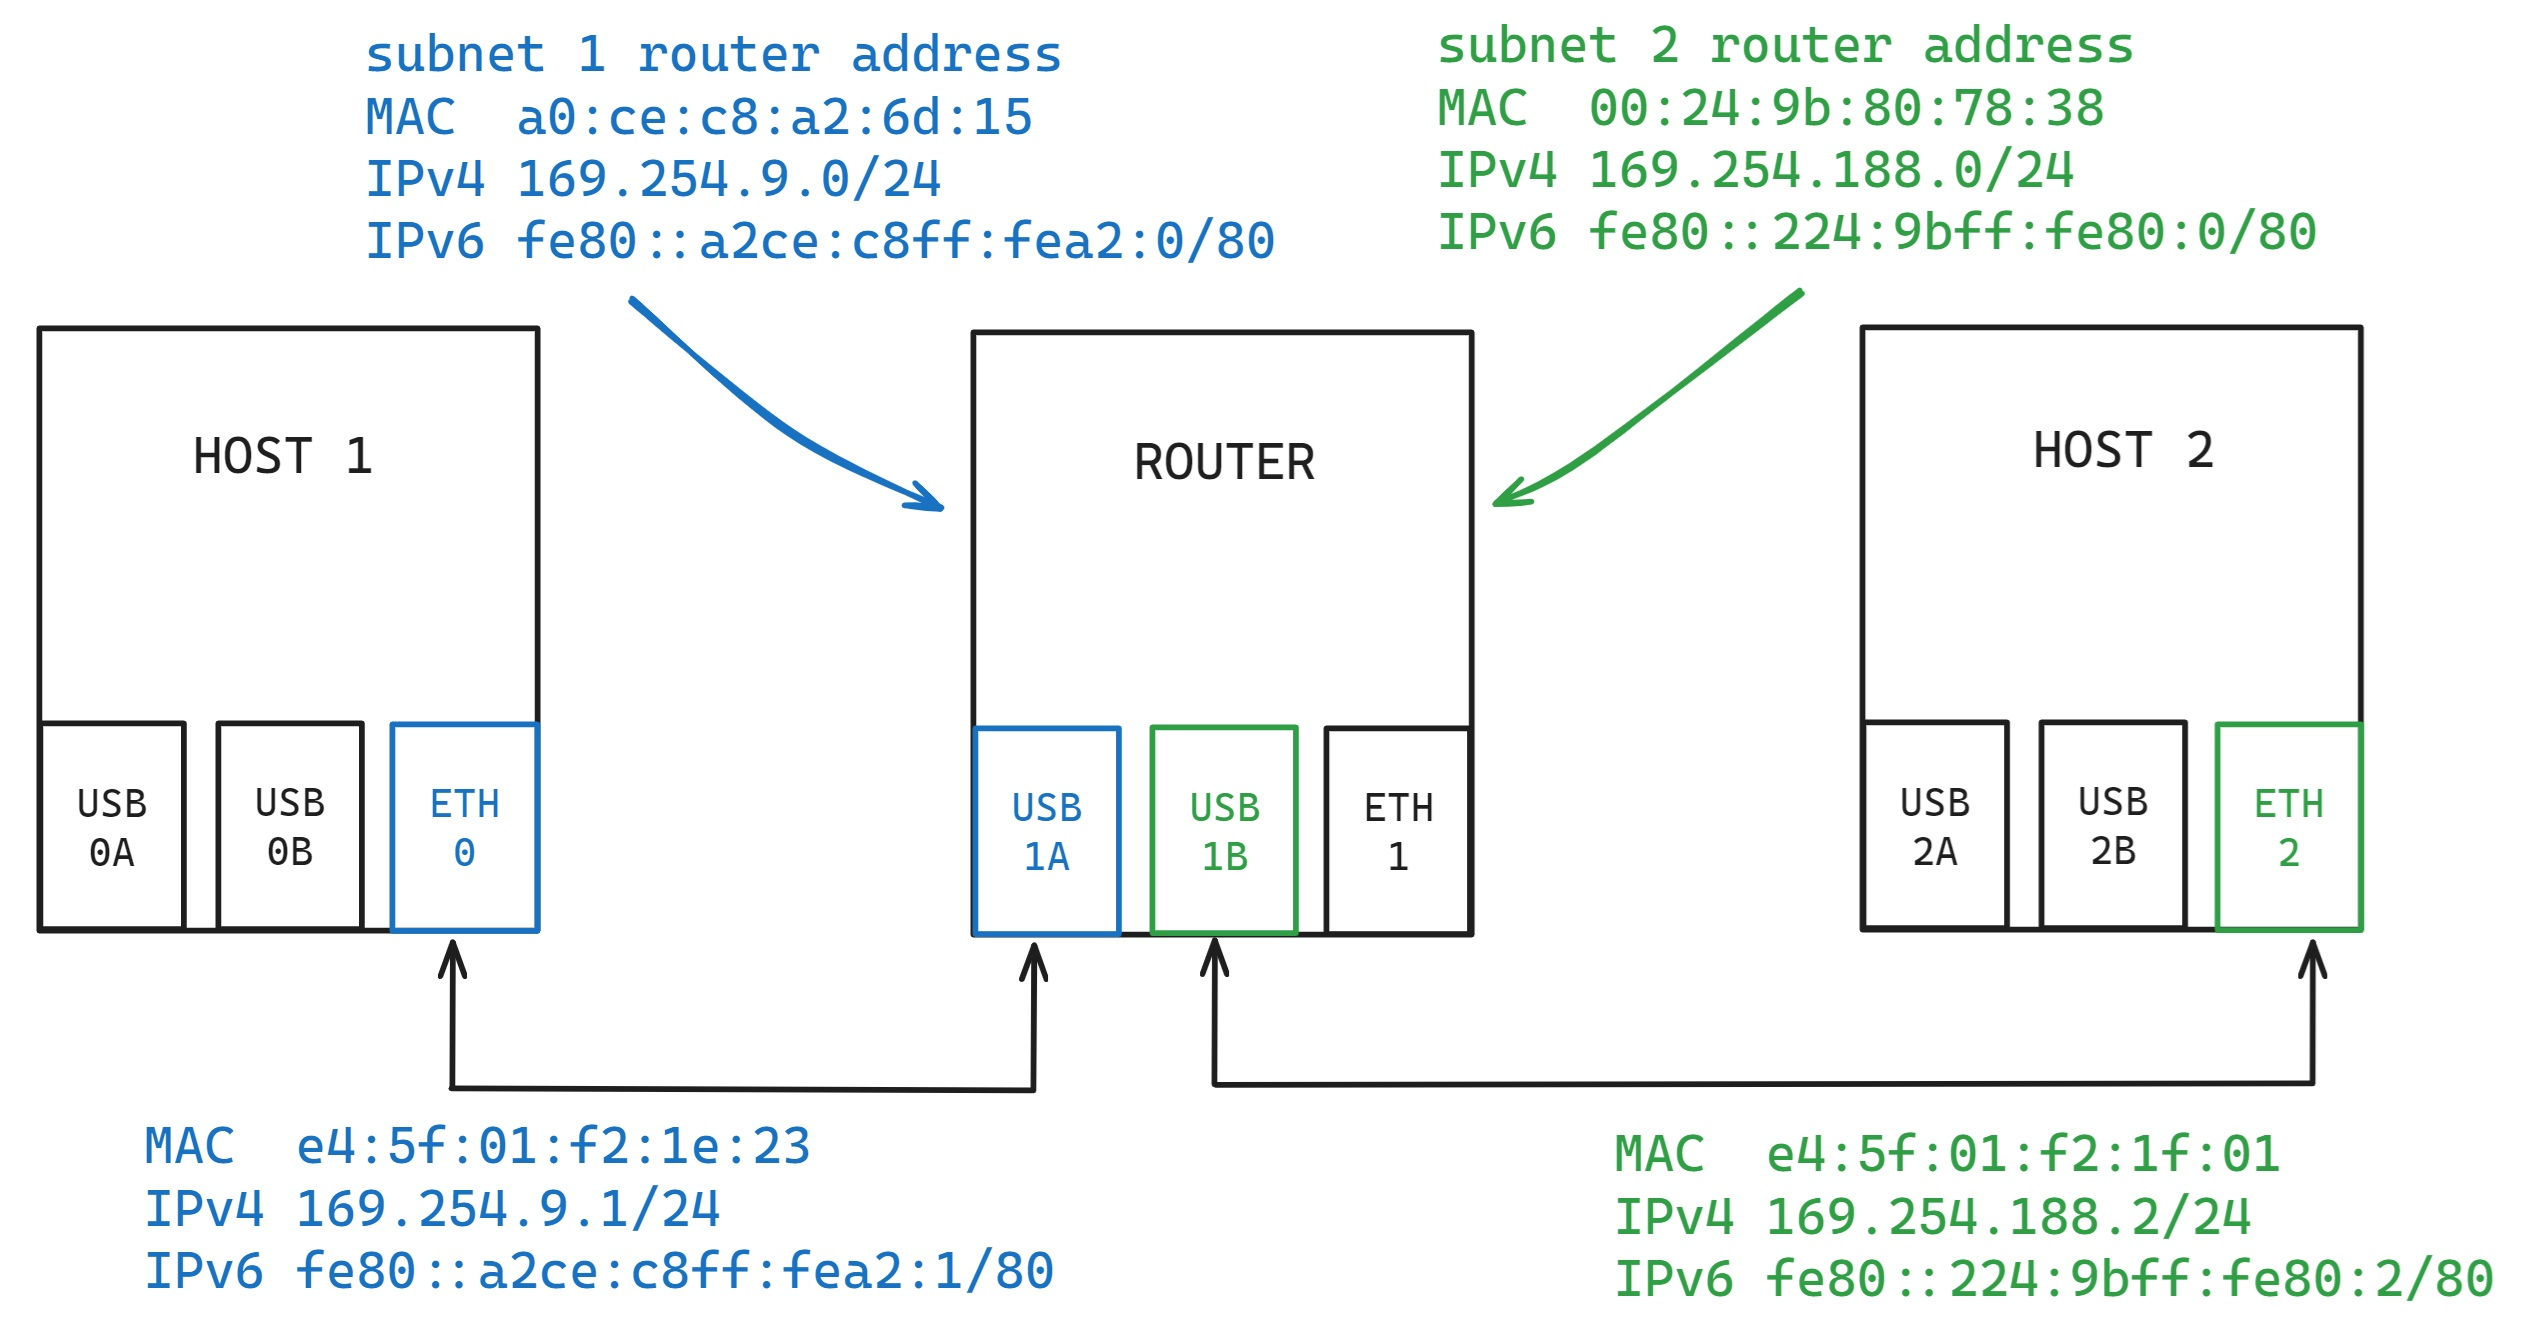
\includegraphics[width=0.85\textwidth]{figures/implementation/setup.jpg}
     \caption{Raspberry Pi setup for the router experiments.}
     \label{fig:impl-setup}
\end{figure}

\pagebreak

\section{Repository Overview}
\label{sec:3.2}

There are a total of eight folders in my code repository, along with a \texttt{README} file. Six of the folders contain a \texttt{.p4} file with the P4 program implementing data plane functionalities, usually along with \texttt{.txt} files with commands to populate the tables in the P4 program through the CLI (effectively acting as the control plane). The seventh repository folder has a Python script I used to plot the graphs in \cref{sec:4.3}. The final repository folder contains the \texttt{LaTeX} source code for my dissertation write up.

\bigskip

\dirtree{%
.1 partii\_dissertation.
.2 README.md.
.2 ipv6 \DTcomment{\textbf{core:} IPv6 forwarding}.
.3 ipv6.p4.
.3 commands.txt.
.2 icmpv6 \DTcomment{\textbf{extension 1:} ICMPv6 functionalities}.
.3 icmpv6.p4.
.2 ndp \DTcomment{\textbf{extension 2:} NDP functionalities}.
.3 ndp.p4.
.3 commands.txt.
.2 router4 \DTcomment{integrates IPv4 functionalities from P4Pi repository}.
.3 router4.p4.
.3 commands.txt.
.2 router6 \DTcomment{integrates IPv6 functionalities from core, extensions 1 and 2}.
.3 router.p4.
.3 commands.txt.
.2 dualstack \DTcomment{\textbf{extension 3:} merges IPv4 and IPv6 functionalities}.
.3 dualstack.p4.
.3 commands.txt.
.2 figures \DTcomment{plots of gathered evaluation data}.
.3 figures.ipynb.
.3 .png files.
.2 dissertation \DTcomment{dissertation source code}.
}

\pagebreak

\section{Implementation Process}
\label{sec:3.3}

I build my IPv6 router prototype using an incremental approach. I implement P4 programs that support independent functionalities, test them in isolation, and then add them to the router. Every P4 program adheres to the \textit{V1Model} architecture model, as outlined in \cref{sec:2.4.1}.

A program adhering to the \textit{V1Model} is comprised of eight distinct code blocks: the header definitions; six packet-processing pipeline stages (parser, checksum verification, ingress processing, egress processing, checksum update, and deparser); and the switch definition. It is not necessary to use all pipeline stages in order to implement a functionality. For example, IPv6 does not use checksums, so those code blocks would be left empty. There are a few characteristics that all my programs share:

\textbf{Ingress Processing} ~ Ingress processing is made up of three different functional blocks: table matchings, actions, and the application block. The application block defines a control flow that decides which action is applied to a packet based on its header fields. Some packets have a table matching performed on a certain header field in order to determine which action is applied to them. Actions include manipulating header fields, choosing egress ports, or simply dropping the packet.

\textbf{Egress Processing} ~ Egress processing is structured the same way as ingress processing. The reason they are separate pipeline stages is that packets that are cloned, recirculated, or generated by the control plane only go through egress processing. For the purposes of this project, all packets go through ingress processing, so I do not require separate egress processing. This pipeline stage is therefore left empty, and I do not mention it again in the following sections.

\textbf{Switch Definition} ~ In every program, the switch definiton takes the six pipeline stage functions as arguments in order to produce a P4 \textit{V1Model} software switch configuration.

In each of the following sections, I describe a functionality design and implementation. I base my designs on observed packet behaviour in a working home network and developed my router such that it mimics the behaviour of my home router. All program logic is my own work.



\section{IPv6 Forwarding}
\label{sec:3.4}

The core objective of my project is to implement the necessary components of an IPv6 router: parsing and forwarding. My P4 program parses an incoming packet, does a longest prefix match on the destination address, and, if there is a table hit, forwards the packet to a specified port.



\subsection{IPv6 Header Packet Format}
\label{sec:3.4.1}

The IPv6 header format is 40 bytes long and made up of 8 fields, as shown in \cref{fig:impl-ipv6header}. For the purposes of this project, aside from the Destination Address field, I reference the Next Header field, used to identify the type of payload being carried by the packet, and the Hop Limit field, used to indicate when a packet has exceeded the amount of nodes it is allowed to visit in the network before it is dropped. The packet's payload is appended to the end of the IPv6 header.

\begin{figure}[htbp]
  \centering
    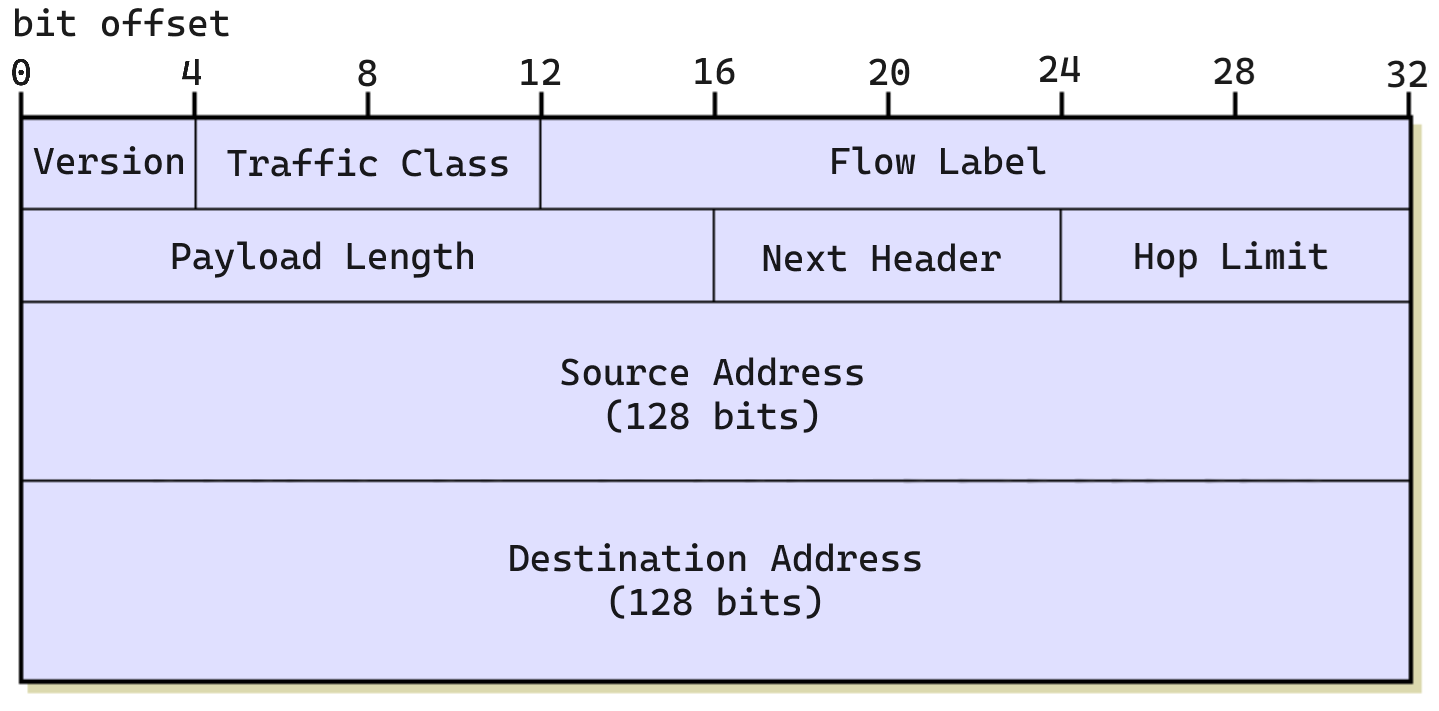
\includegraphics[width=0.55\textwidth]{figures/implementation/ipv6_header.png}
    \caption{IPv6 header format. Adapted from \cite{IPguide}.}
    \label{fig:impl-ipv6header}
\end{figure}



\subsection{IPv6 Forwarding Design}
\label{sec:3.4.2}

Once the data plane is configured, I populate the IPv6 forwarding table using the CLI. The entries use IPv6 addresses as keys, which match to a next-hop MAC address and a port output number. A packet sent from Host 1 is forwarded by the router towards Host 2, and vice versa. No packet loss or duplication is observed. For more detailed information on how to run this experiment, consult Appendix C.



\subsection{IPv6 Forwarding Program}
\label{sec:3.4.3}

The data plane behaviour of the router is specified by the P4 file \texttt{ipv6.p4}. 

\textbf{Header Definitions} ~ I define two header types: a 14-byte Ethernet header, which contains a source MAC address, a destination MAC address, and a Type field; and a 40-byte IPv6 header, which contains Version, Traffic Class, Flow Label, Payload Length, Next Header, and Hop Limit fields, together with a source and destination IPv6 address.

\textbf{Parser} ~ The parser filters incoming packets based on their headers. This program’s parser state machine has two intermediary states: one for parsing Ethernet headers and one for parsing IPv6 headers, as shown in \cref{fig:impl-ipv6parser}. The \texttt{start} state automatically transitions to the \texttt{Ethernet} state, where the Ethernet header is extracted and a check is performed, testing whether the next header is of type IPv6. If it is, the state machine transitions to the \texttt{IPv6} state. There it extracts the IPv6 header and moves on to the next stage of the \textit{V1Model} pipeline.

\begin{figure}[htbp]
  \centering
    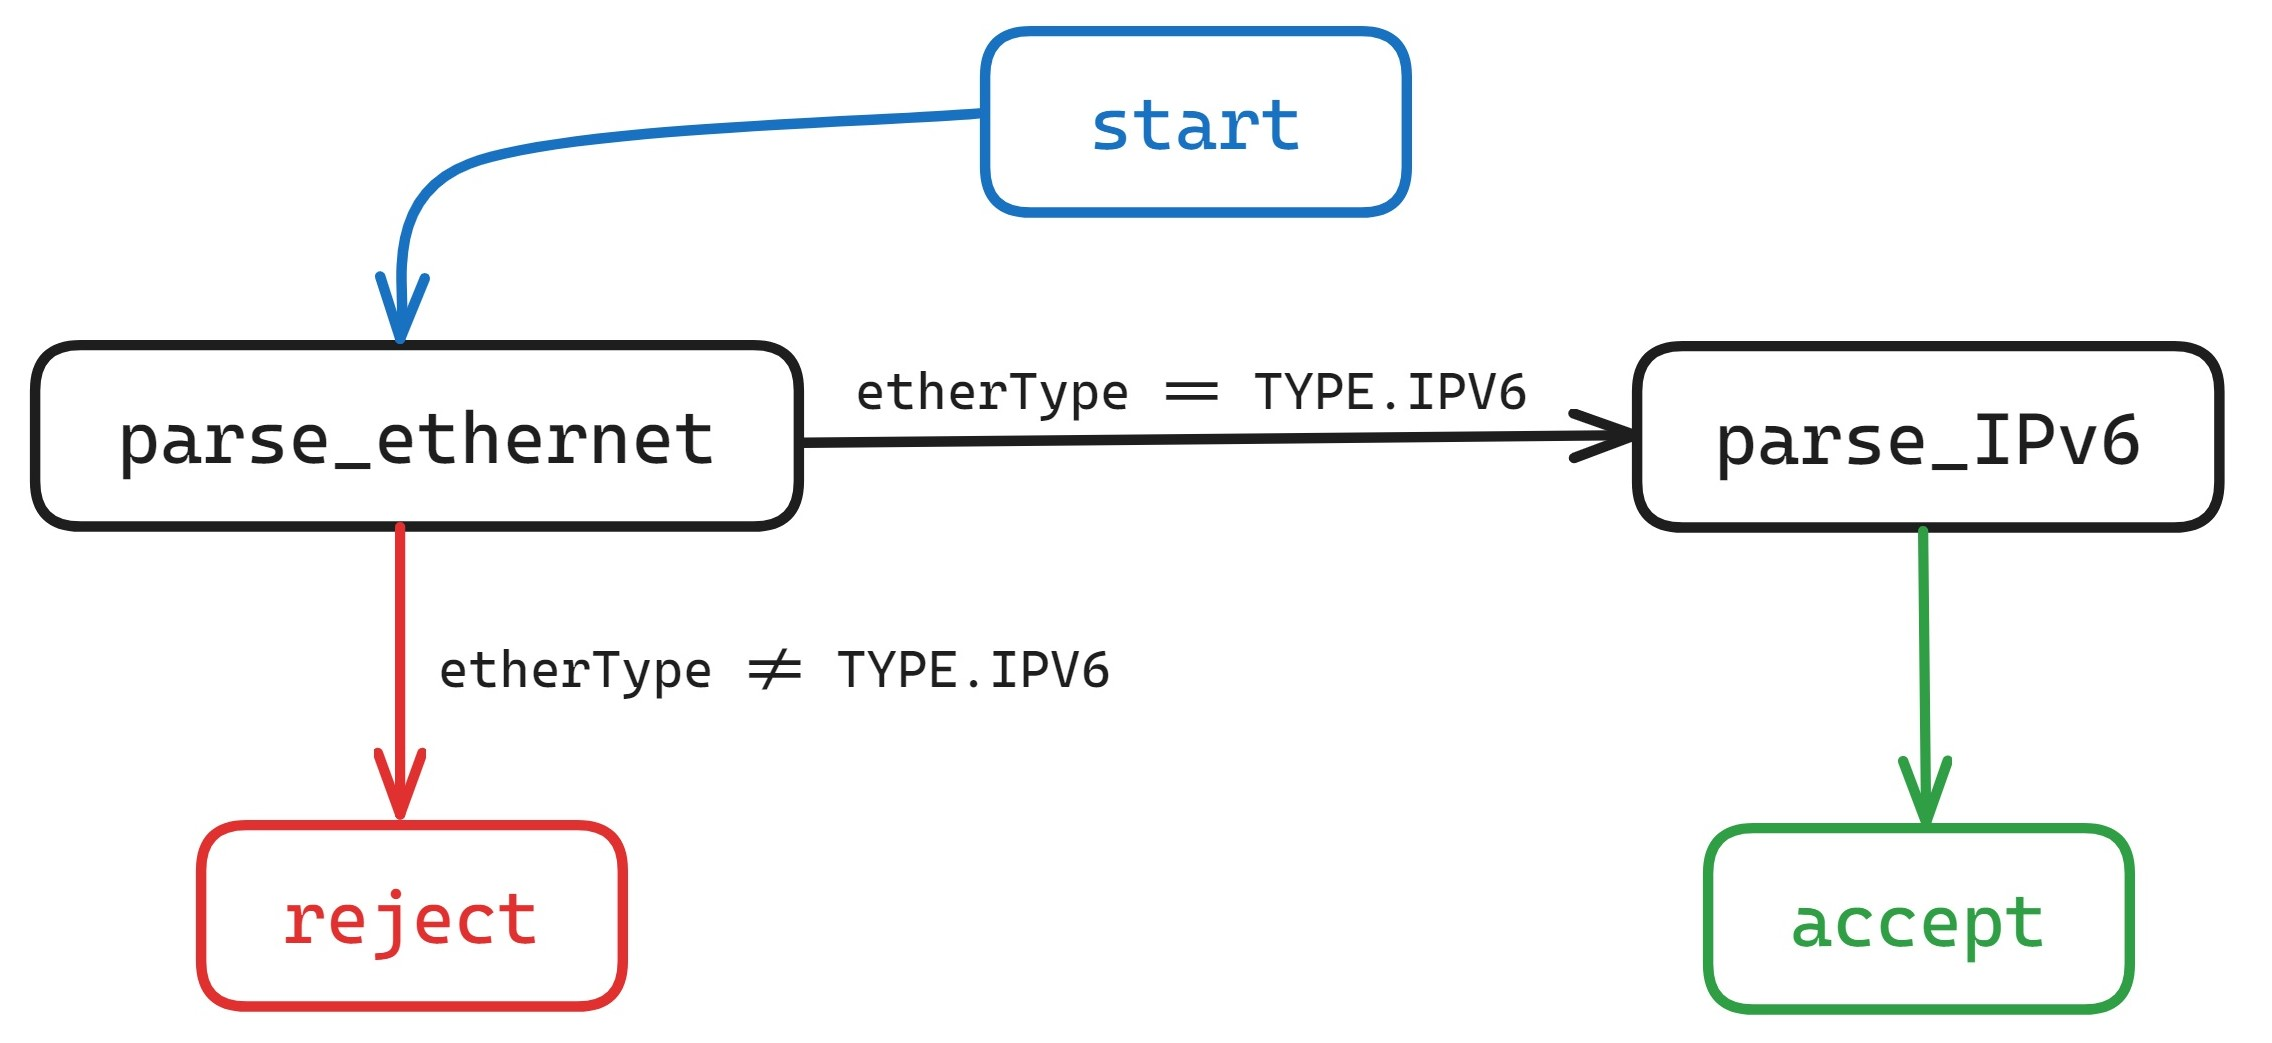
\includegraphics[width=0.6\textwidth]{figures/implementation/ipv6_parser.jpg}
     \caption{IPv6 forwarding parser state machine diagram.}
     \label{fig:impl-ipv6parser}
\end{figure}

\textbf{Checksum Verification} ~ IPv6 does not use checksums, so this pipeline stage is unused, and the code block is left empty.

\textbf{Ingress Processing} ~ Since we only have IPv6 forwarding, the control flow is relatively simple. It is illustrated in \cref{fig:impl-ipv6apply}, where a packet will either be forwarded or dropped, based on its header fields and the data plane's table entries. If the Hop Limit is larger than one, a longest prefix match is performed on the destination address of the packet. If a match is found, the IPv6 forward action is called, which assigns an output port, updates the Ethernet’s source and destination addresses based on the next hop to be taken, and decrements the IPv6 Hop Limit field. A code snippet of the IPv6 forwarding action can be seen in \cref{fig:impl-ipv6forward}.

\begin{figure}[htbp]
  \centering
    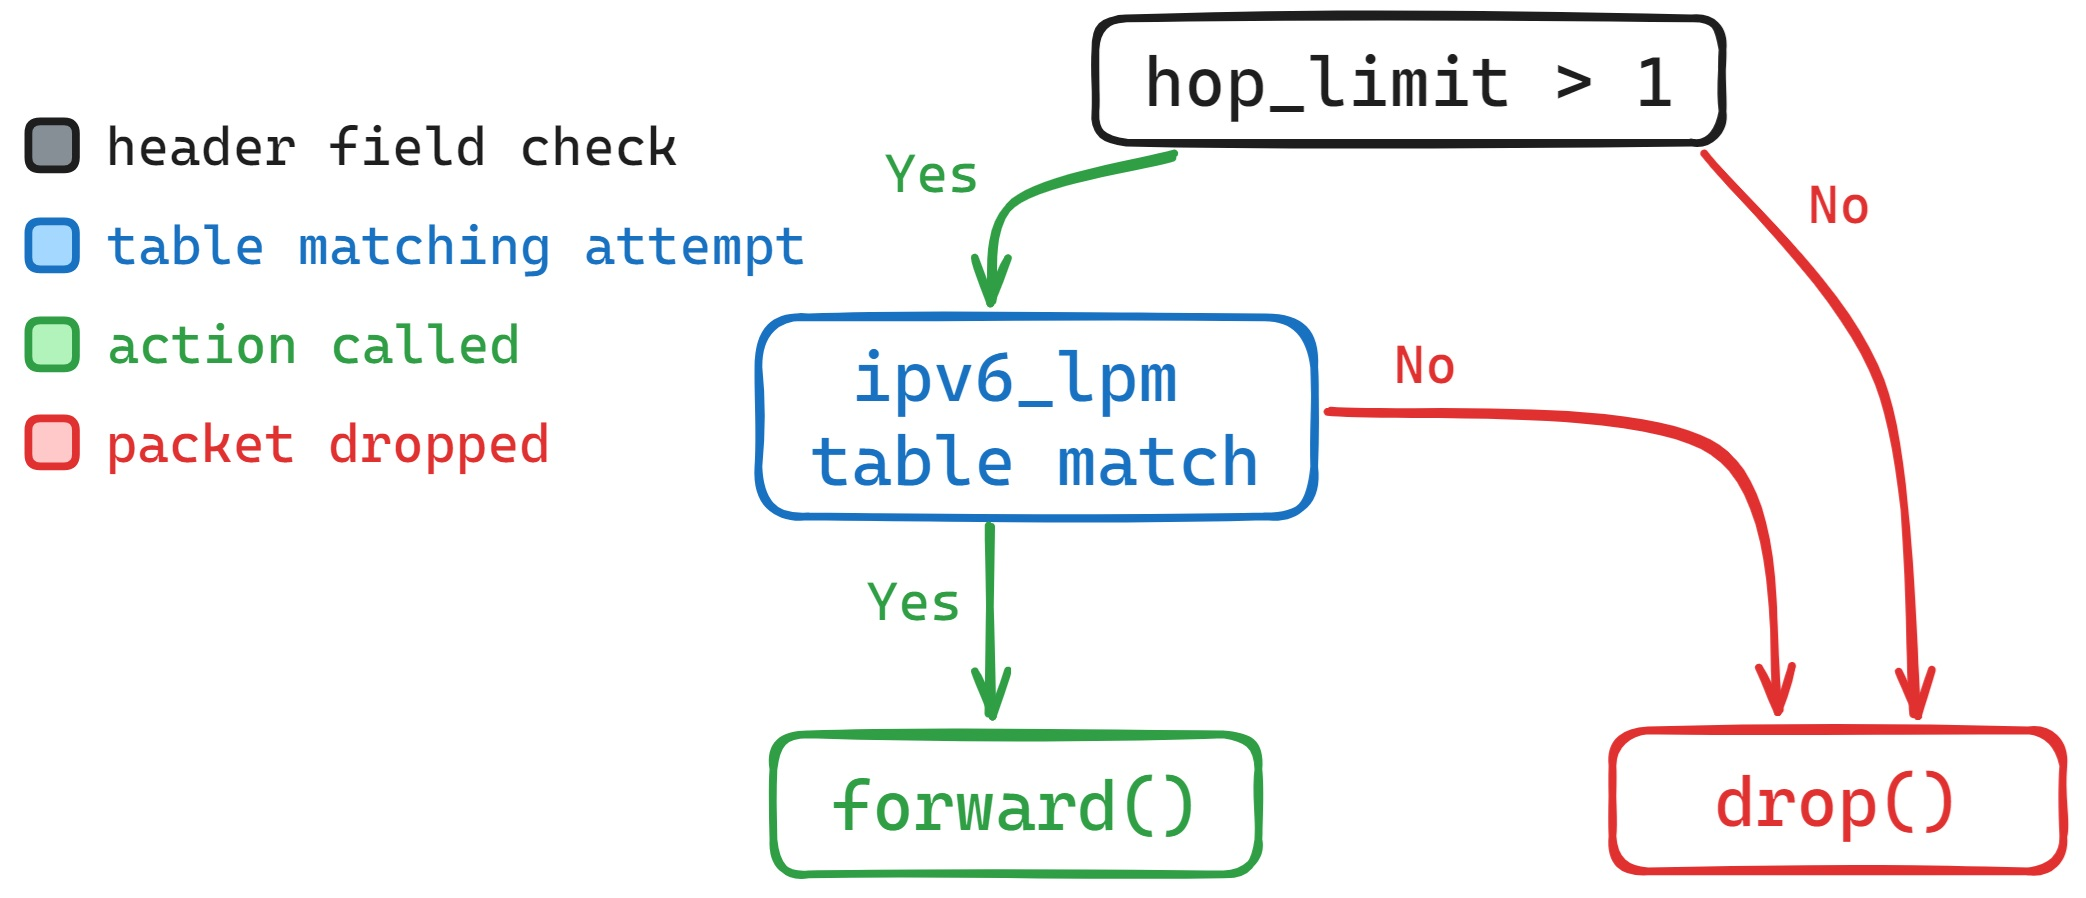
\includegraphics[width=0.6\textwidth]{figures/implementation/ipv6_apply.jpg}
     \caption{IPv6 forwarding control flow represented as a simplified decision tree.}
     \label{fig:impl-ipv6apply}
\end{figure}

\begin{figure}[htbp]
  \centering
    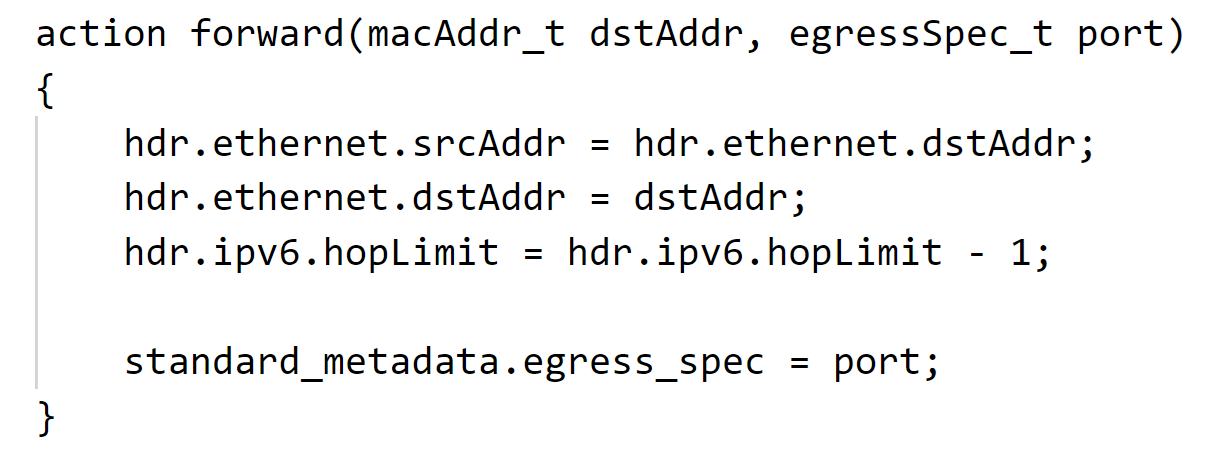
\includegraphics[width=0.6\textwidth]{figures/implementation/ipv6_forward.png}
     \caption{IPv6 forwarding action code block.}
     \label{fig:impl-ipv6forward}
\end{figure}

\textbf{Checksum Calculation} ~ Once again, this pipeline stage is unused.

\textbf{Deparser} ~ The payload proceeds to the deparser stage, where the updated headers are prepended before it is sent out of the router through the assigned egress port.

This program provides functionalities required for parsing, table matching, and forwarding IPv6 packets from one subnet to another. The two hosts are able to discover each other on the network and exchange packets. This fulfils my project's core objectives.


\section{ICMPv6 (Internet Control Message Protocol)}
\label{sec:3.5}

The first extension in my project is to implement ICMPv6 functionalities. ICMPv6 is used to report network errors and provide diagnostic functions. To demonstrate that core ICMPv6 functionalities work, I implement four of the most common messages. Specifically, I implement two informational messages (Echo Request/Reply) and two error messages (Destination Unreachable and Time Exceeded). 



\subsection{ICMPv6 Packet Formats}
\label{sec:3.5.1}

ICMPv6 packets are encapsulated in an IPv6 payload. They all have Type, Code and Checksum fields, but the rest of the packet differs depending on the specific message being relayed. Even though IPv6 does not have checksums, ICMPv6 does. ICMPv6 checksums are calculated using an IPv6 pseudoheader \cite{ICMPv6Specs}. The Echo Reply and Echo Response packets have optional data such as a timestamp, and the error messages have a payload containing the first bytes of the original packet that triggered the error. The formats of the Echo Request/Reply, Time Exceeded packets, and Destination Unreachable are shown in \cref{fig:impl-echoheader}, \cref{fig:impl-timeexheader}, and \cref{fig:impl-destunrheader}, respectively.

\begin{figure}[htbp]
\begin{subfigure}{\textwidth}
  \centering
  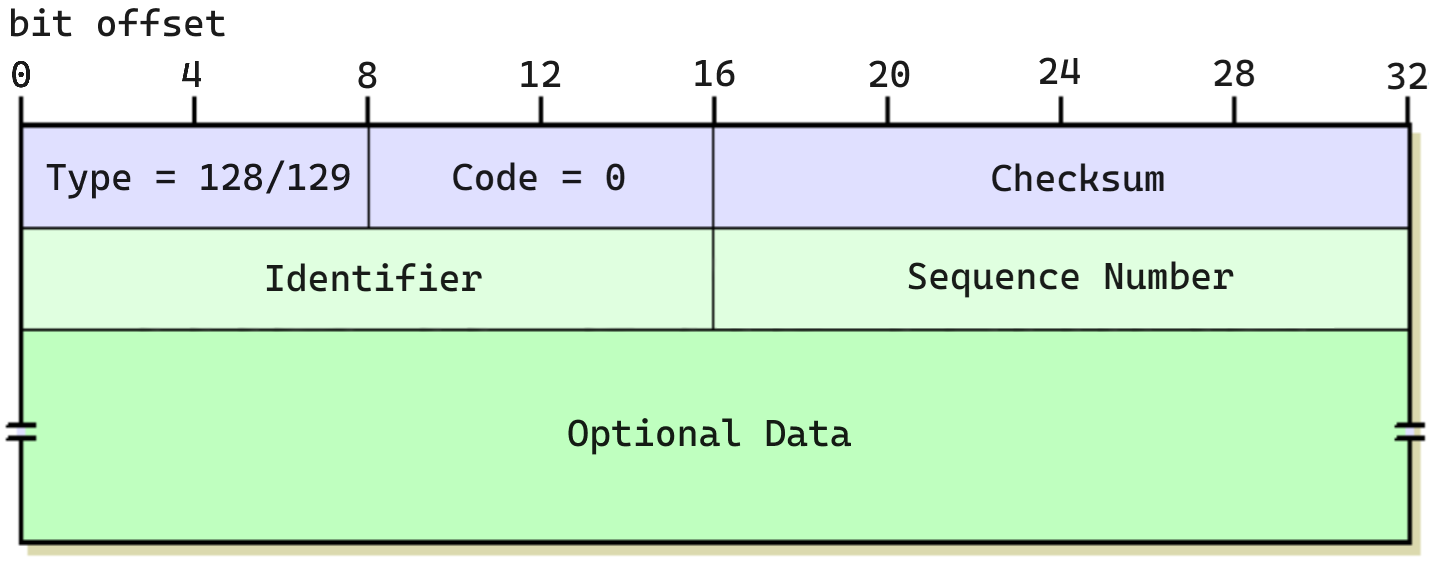
\includegraphics[width=0.5\textwidth]{figures/implementation/icmpv6_echo.png}
  \caption{Echo Request/Reply.}
  \label{fig:impl-echoheader}
\end{subfigure}
\par \medskip
\begin{subfigure}{.5\textwidth}
  \centering
  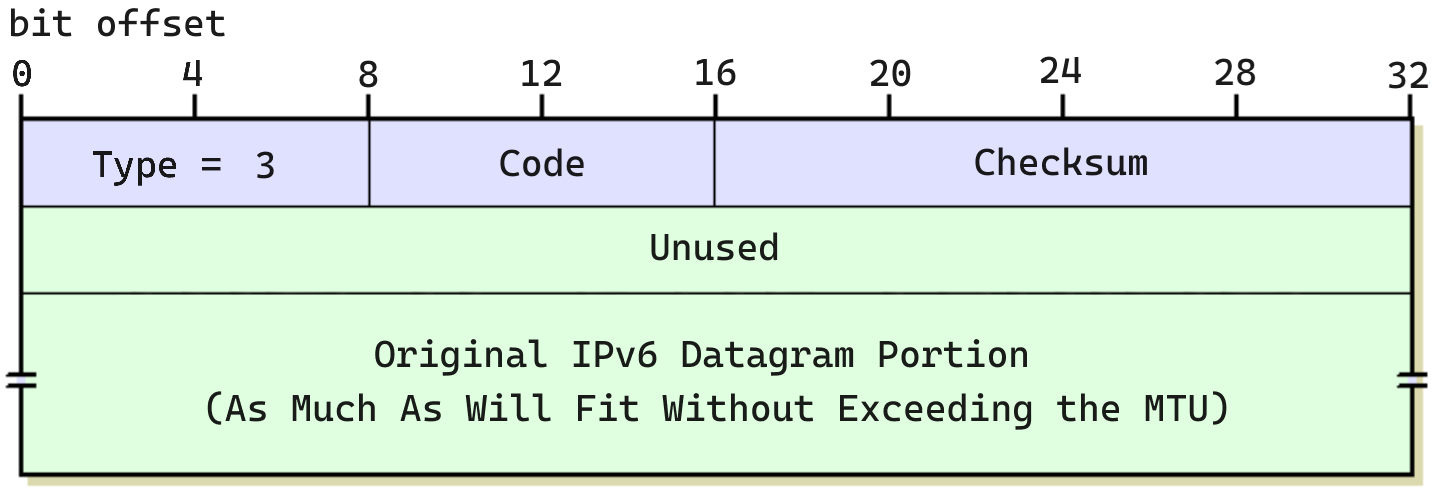
\includegraphics[width=1\textwidth]{figures/implementation/icmpv6_timeexceeded.png}
  \caption{Time Exceeded.}
  \label{fig:impl-timeexheader}
\end{subfigure}%
\begin{subfigure}{.5\textwidth}
  \centering
  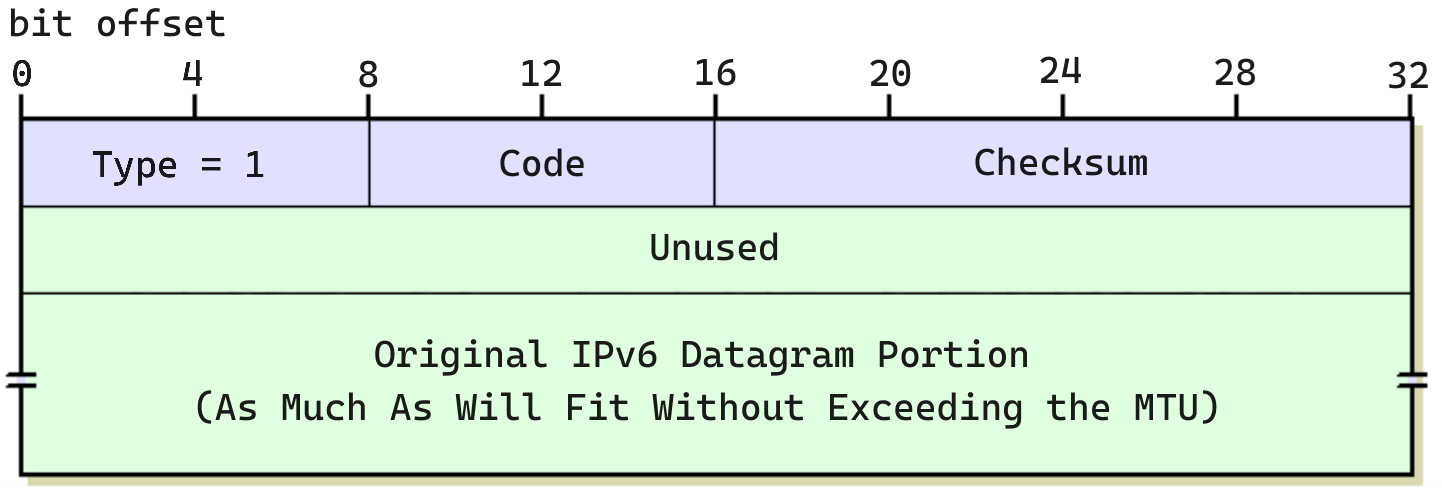
\includegraphics[width=1\textwidth]{figures/implementation/icmpv6_destunreachable.png}
  \caption{Destination Unreachable.}
  \label{fig:impl-destunrheader}
\end{subfigure}
\caption{ICMPv6 packet formats. Adapted from \cite{IPguide}.}
\label{fig:test}
\end{figure}


\subsection{ICMPv6 Design}
\label{sec:3.5.2}

An Echo Request directed at a defined router address receives an Echo Reply. A Destination Unreachable error message is generated if the destination address of the Echo Request is unknown to the router, and a Time Exceeded error message is generated if the Echo Request reaches the router with a remaining Hop Limit of zero or one. For more detailed information on how to run this experiment, consult Appendix D.

I design the program such that it can trivially be extended to support other ICMPv6 messages. For example, a packet with a malformed header would not pass a header validity test in the program. If that happens, the current design of the router would drop the packet. Instead, a new action could be defined to return a Parameter Problem error message.



\subsection{ICMPv6 Program}
\label{sec:3.5.3}

The data plane behaviour of the router is defined by the P4 file \texttt{icmpv6.p4}.

\textbf{Header Definitions} ~ I define two additional header types: a 4-byte ICMPv6 header, which contains Type, Code, and Checksum fields; and a 60-byte Echo header, which contains Identifier and Sequence Number fields, and a payload for the optional data.

\textbf{Parser} ~ The parser state machine of this program reflects the addition of the ICMPv6 and Echo headers and only accepts packets that are Echo Requests. It identifies these packets by checking the Next Header field in the extracted IPv6 header, and the Type field of the ICMPv6 header. The parser state machine diagram is shown in \cref{fig:impl-icmpv6parser}.

\begin{figure}[htbp]
  \centering
    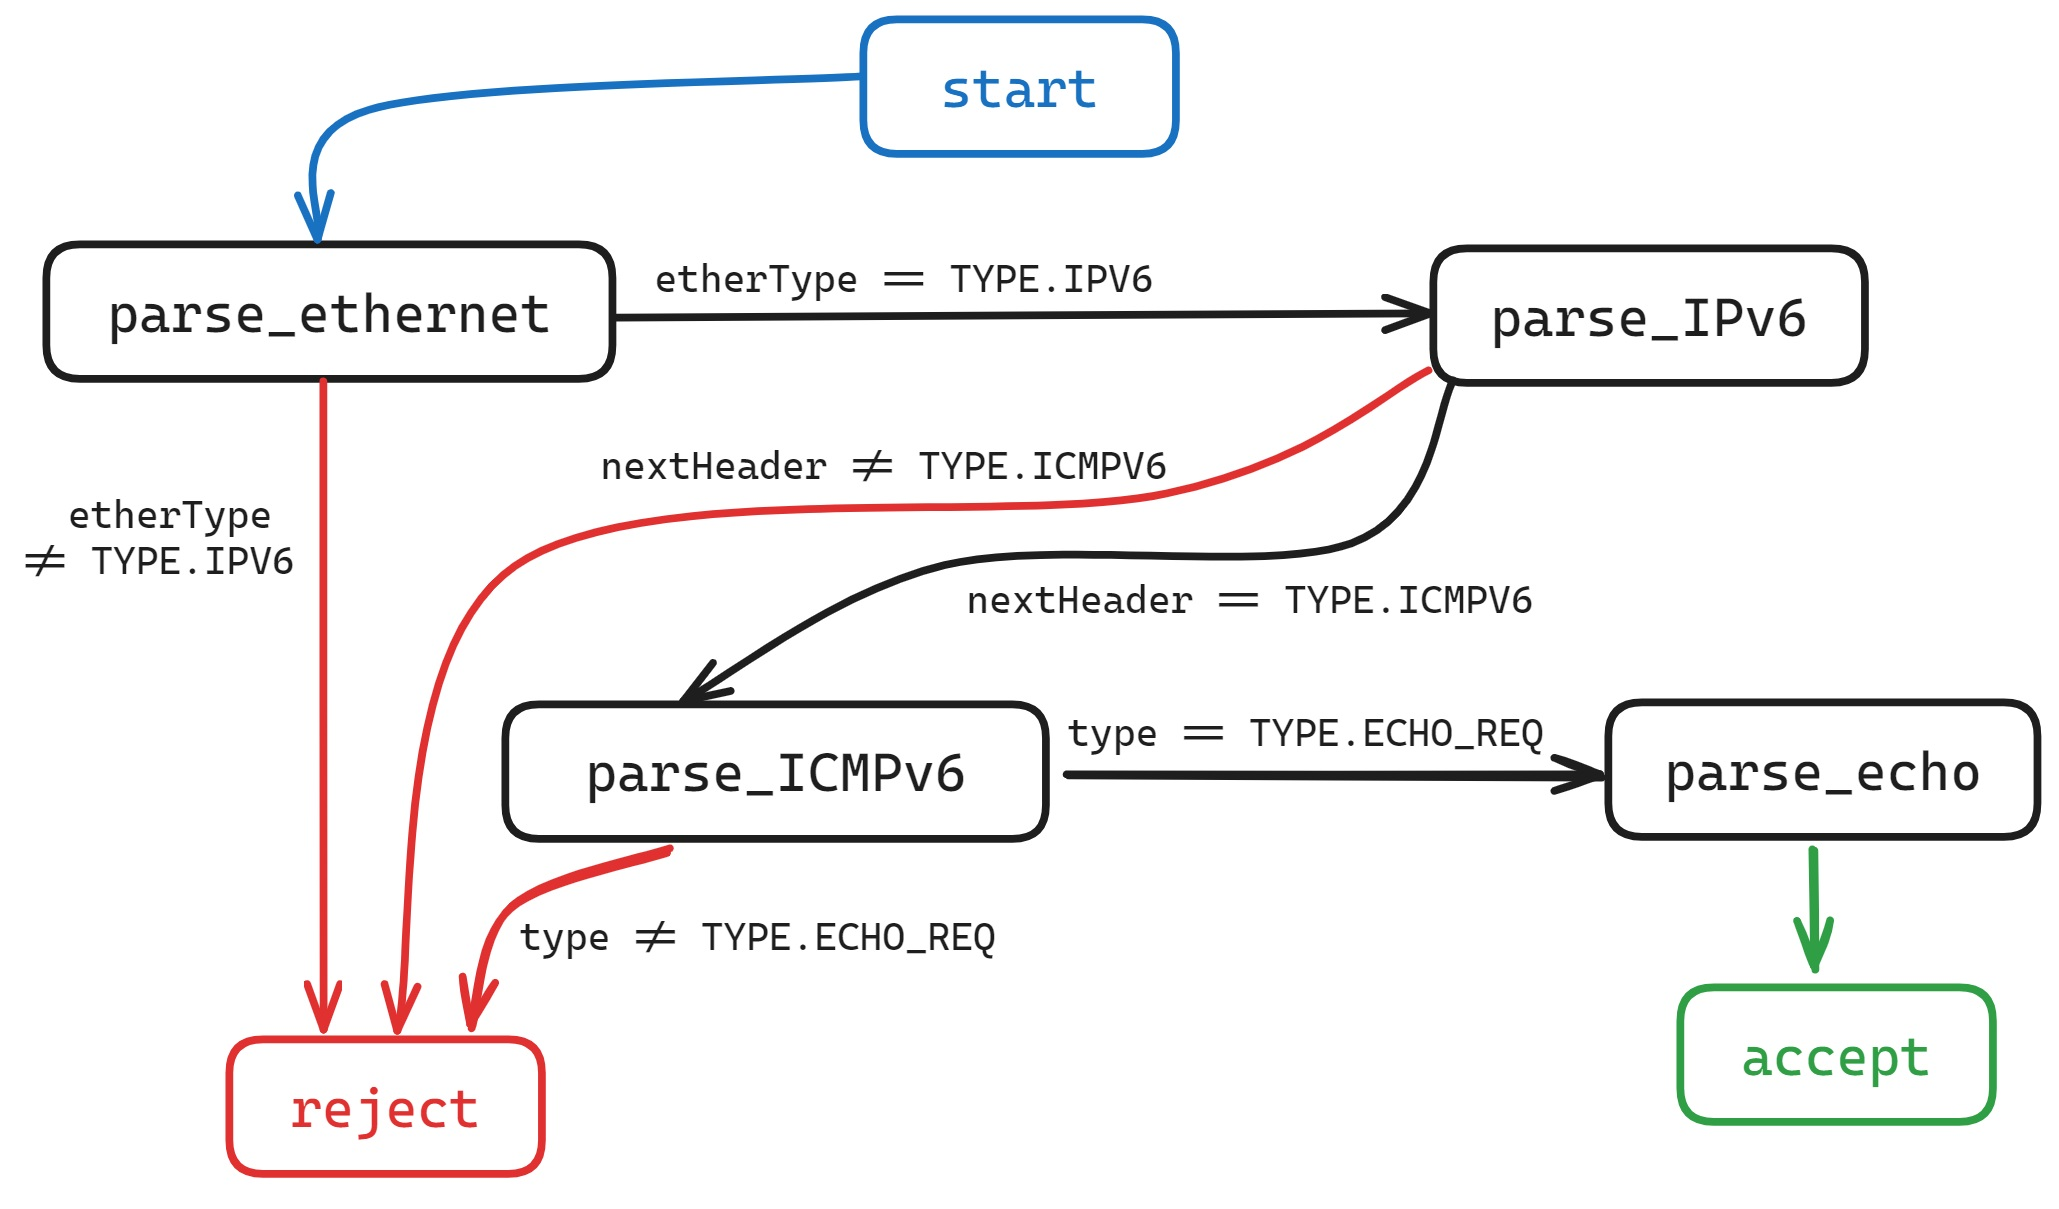
\includegraphics[width=0.70\textwidth]{figures/implementation/icmpv6_parser.jpg}
     \caption{ICMPv6 parser state machine diagram.}
     \label{fig:impl-icmpv6parser}
\end{figure}

\textbf{Checksum Verification} ~ The ICMPv6 checksum is verified before the packet proceeds to ingress control blocks. ICMPv6 checksums are calculated using all fields in the ICMPv6 packet, along with an IPv6 pseudoheader, made up of the source and destination addresses, the payload length, and the Next Header field value. The checksum function splits the data into 16-bit pieces and one's complement sums all of them by carrying the one if the sum overflows. The checksum is then the 16 bit one's complement of the result.

\textbf{Ingress Processing} ~ The first performed check is on the Hop Limit -- if it is less than or equal to one, the Time Exceeded action is called. If it is larger than one, the next check is on the ICMPv6 Type field. Even though this program's parser only accepts packets of type Echo Request, I added this redundant check for easier integration into the IPv6 router. If the packet is of type Echo Request, the destination address is checked in the Echo Responder table, otherwise it is dropped. The Echo Responder table matches the address to its statically defined entries (the router’s addresses) in the P4 program. If a match is found in the table, the Echo Reply action is called, otherwise the Destination Unreachable action is triggered. For both error messages, a longest prefix match table is used to identify which subnet the packet came from in order to send the error message from the respective router IPv6 address and towards the respective subnet’s port. The control flow of the ingress block is shown in \cref{fig:impl-icmpv6apply}.

\begin{figure}[htbp]
  \centering
    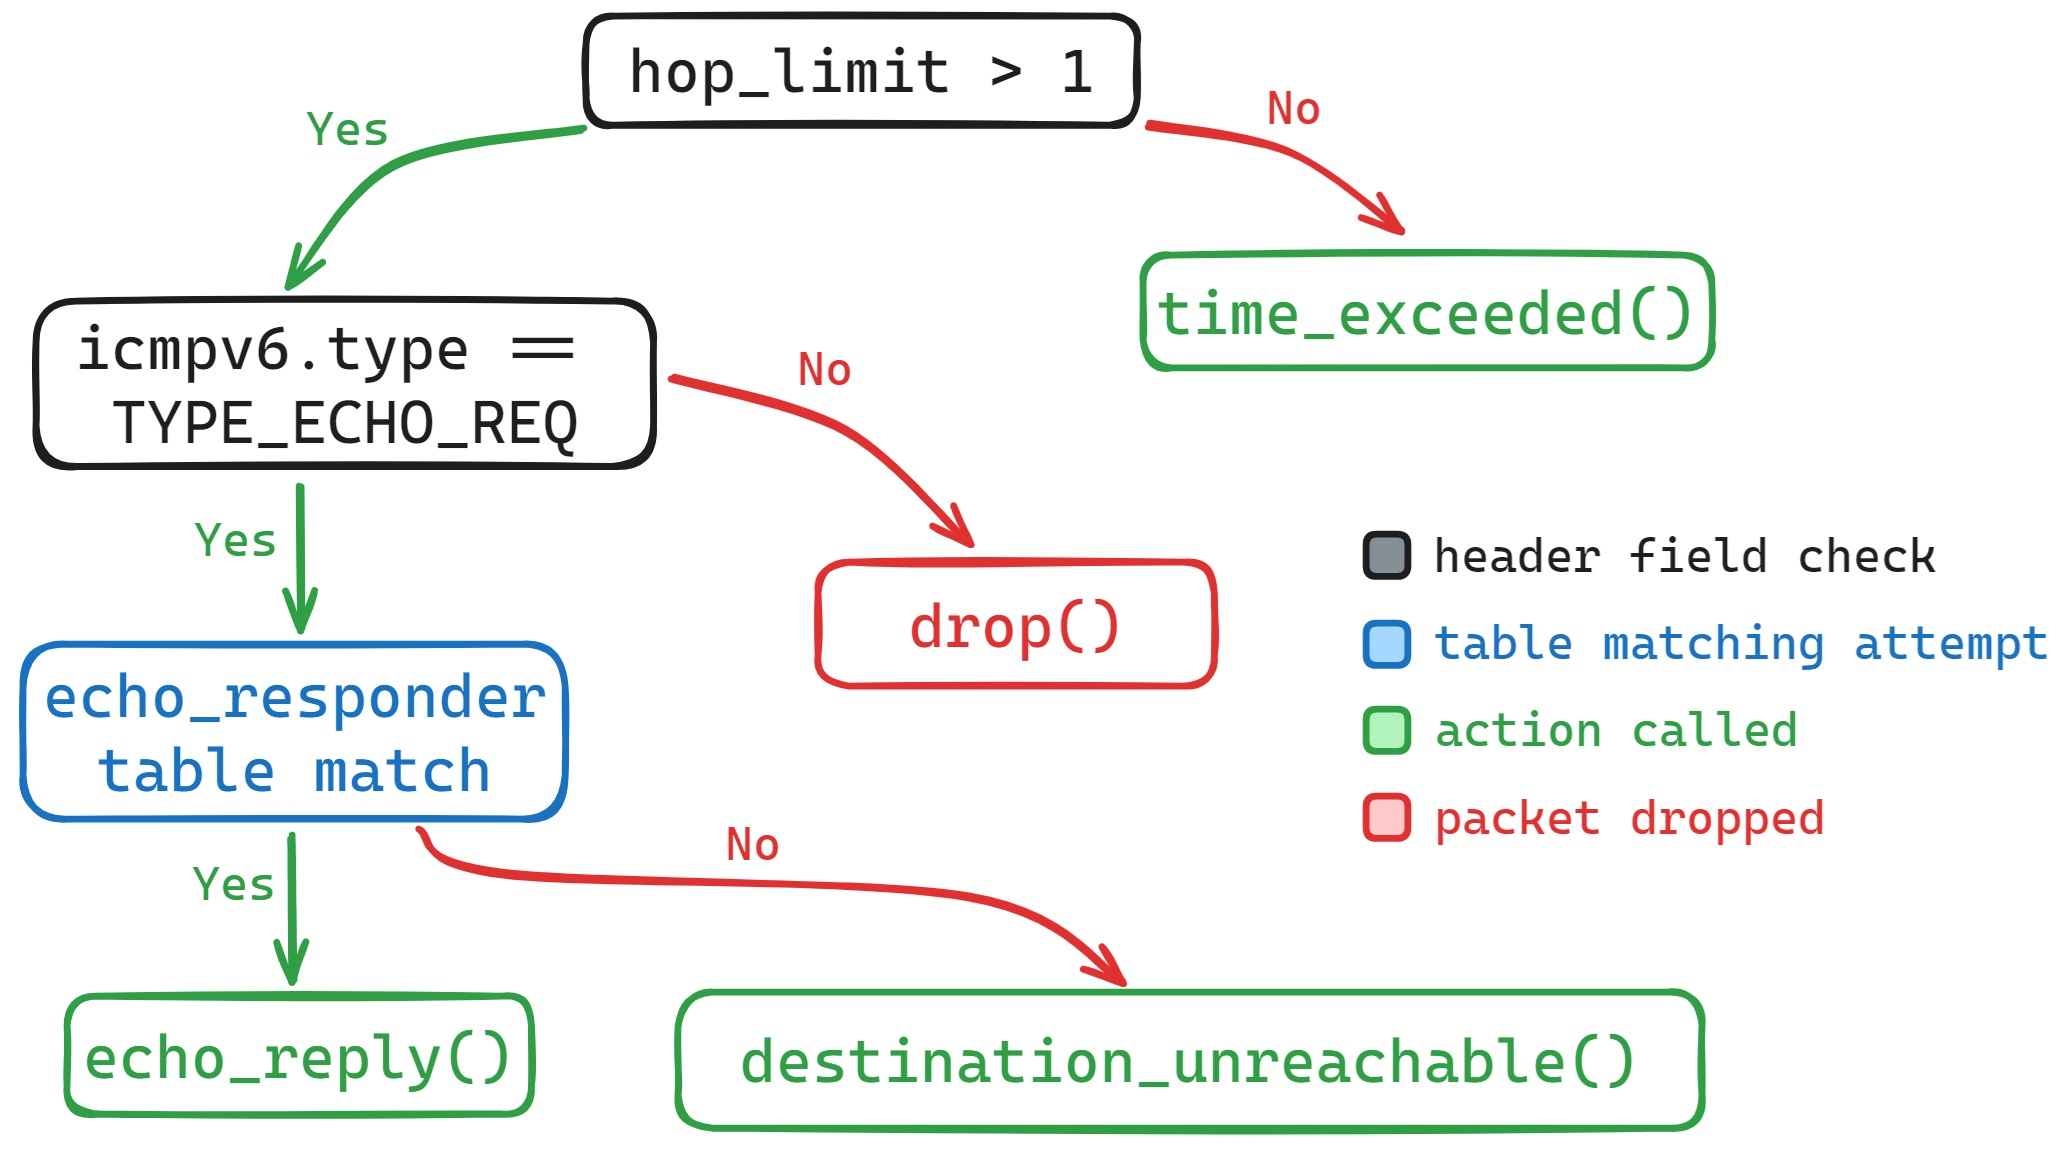
\includegraphics[width=0.65\textwidth]{figures/implementation/icmpv6_apply.jpg}
     \caption{ICMPv6 control flow represented as a simplified decision tree.}
     \label{fig:impl-icmpv6apply}
\end{figure}

When an action is called, the Type field of the ICMPv6 packet is updated accordingly. For an Echo Response no other ICMPv6 fields are modified. For generating error messages, the packet payload is updated to the original packet's dataframe. In all cases, the source addresses of the IPv6 and Ethernet headers are updated to match the corresponding subnet’s router addresses and the destination addresses are set to the original packet’s source addresses. The code block for the Echo Reply action is shown in \cref{fig:impl-icmpv6echoreply}.

\begin{figure}[htbp]
  \centering
    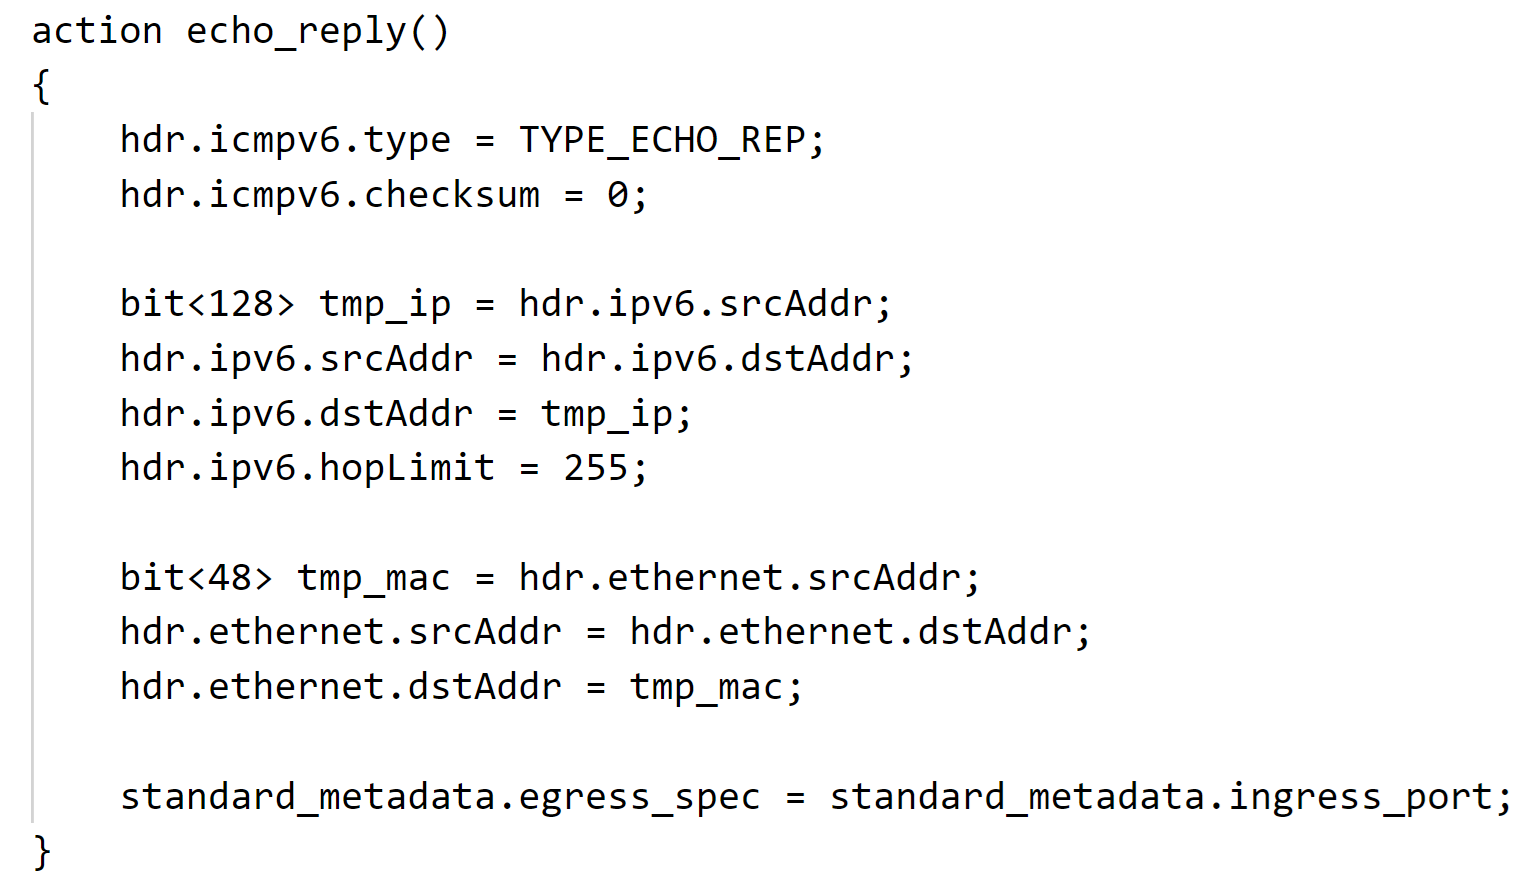
\includegraphics[width=0.7\textwidth]{figures/implementation/icmpv6_echoreply.png}
     \caption{ICMPv6 Echo Reply action code block.}
     \label{fig:impl-icmpv6echoreply}
\end{figure}

\textbf{Checksum Calculation} ~ An ICMPv6 checksum computation is performed using an IPv6 pseudoheader, and the value is placed in the ICMPv6 Checksum field.

\textbf{Deparser} ~ The deparser prepends all headers onto the outgoing packet before sending it out of the specified egress port into the correct subnet.

This program implements core ICMPv6 functionalities and allows for the code to be extended to support other ICMPv6 messages. A host that sends an Echo Request to the router receives an Echo Reply. Any packet that has exceeded the Hop Limit generates a Time Exceeded error message from the router, and any packet whose destination address is not known to the router generates a Destination Unreachable error message. This concludes my first project extension. 



\section{NDP (Neighbour Discovery Protocol)}
\label{sec:3.6}

My second project extension is to implement NDP functionalities. Nodes use NDP to learn about network configurations and nodes' link-layer addresses. In IPv6, Neighbour Discovery happens on top of the network layer, using ICMPv6 messages. There are five different packet types in ICMPv6 that are used for NDP purposes, and I implement two of them -- Neighbour Solicitation (NS) and Neighbour Advertisement (NA) -- to show that my router can support NDP functionalities.



\subsection{NDP Packet Formats}
\label{sec:3.6.1}

NS and NA packets start as all ICMPv6 packets do: with Type, Code and Checksum fields. The remainder of the packet contains 32 reserved bits (three bits of which are used for flags in the NA packet) and the address that needs to be resolved. The NA packet puts the link-layer address of the target IPv6 address in the options field. All NDP packets are encapsulated within an IPv6 payload. NS and NA packet formats can be seen in \cref{fig:impl-ndpsolheader} and \cref{fig:impl-ndpadvheader}, respectively.

\begin{figure}[htbp]
\centering
\begin{subfigure}{.5\textwidth}
  \centering
  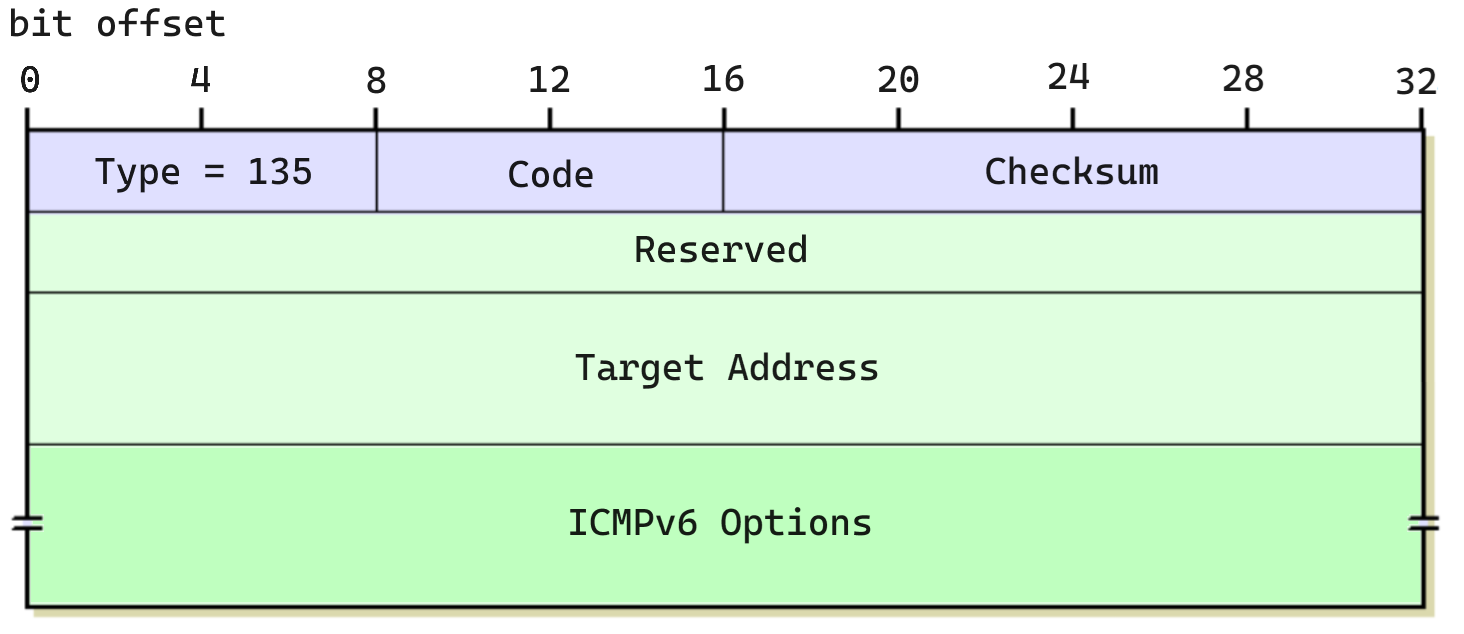
\includegraphics[width=1\linewidth]{figures/implementation/ndp_sol.png}
  \caption{Neighbour Solicitation packet format.}
  \label{fig:impl-ndpsolheader}
\end{subfigure}%
\begin{subfigure}{.5\textwidth}
  \centering
  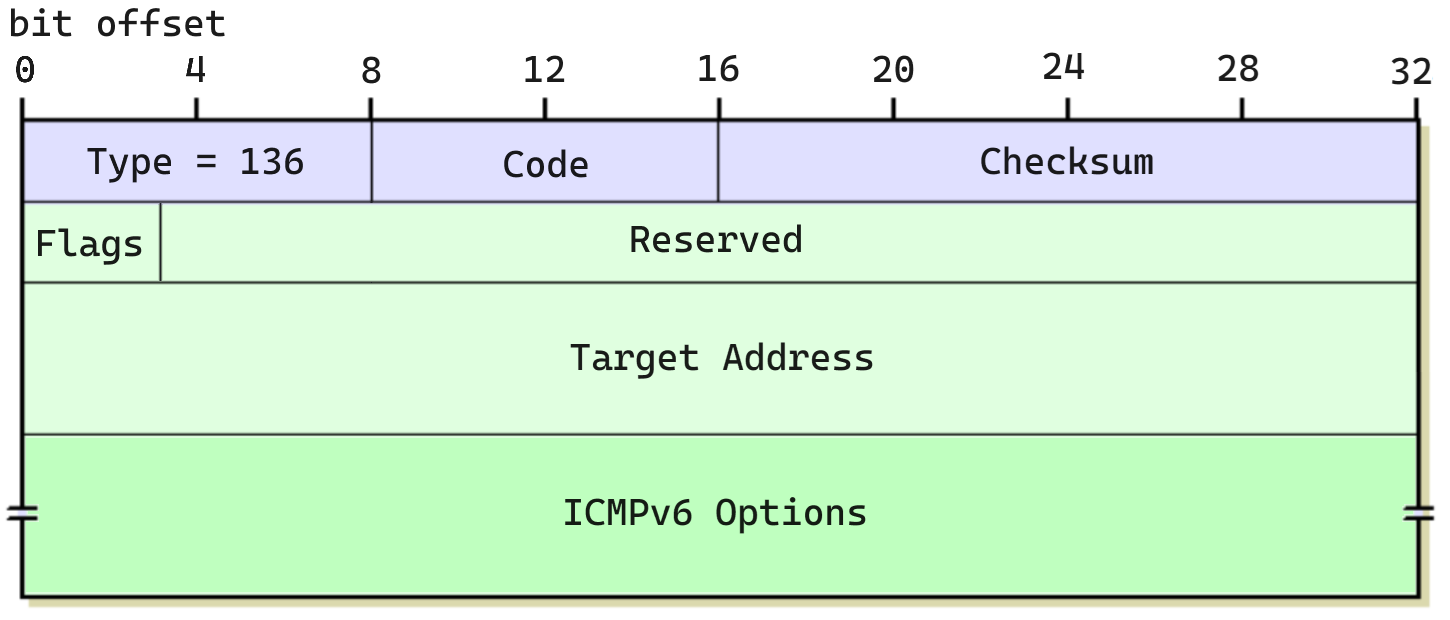
\includegraphics[width=1\linewidth]{figures/implementation/ndp_adv.png}
  \caption{Neighbour Advertisement packet format.}
  \label{fig:impl-ndpadvheader}
\end{subfigure}
\caption{NDP packet formats. Adapted from \cite{IPguide}.}
\label{fig:impl-ndpmsgs}
\end{figure}



\subsection{NDP Design}
\label{sec:3.6.2}

The router's tables are populated with IPv6-MAC address pairs using the CLI. The router responds to any NS whose target address it recognises with an NA that contains the corresponding link-layer address. Since NDP acquires next-hop MAC addresses, I do not manually input any neighbour entries into the hosts, unlike in previous experiments. Issuing Echo Requests results in the hosts’ neighbour tables populating the entries they receive from the router. Appendix E contains details on how to run this experiment. Once again, I design the program in a way that allows for it to trivially be extended to support other NDP messages.



\subsection{NDP Program}
\label{sec:3.6.3}

The data plane behaviour of the router is defined by the P4 file \texttt{ndp.p4}.

\textbf{Header Definitons} ~ I define a new header type in place of the Echo header: a 28-byte Nei header, containing 3 bit flags, reserved bits, a target address, an Options Type field, an Options Length field, and a payload.

\textbf{Parser} ~ The parser state machine of this program, seen in \cref{fig:impl-ndpparser}, is similar to the one in extension 1, \cref{fig:impl-icmpv6parser}, with the \texttt{Echo} state being replaced by the \texttt{Nei} state. Only packets of type NS are accepted by the parser.

\begin{figure}[htbp]
  \centering
    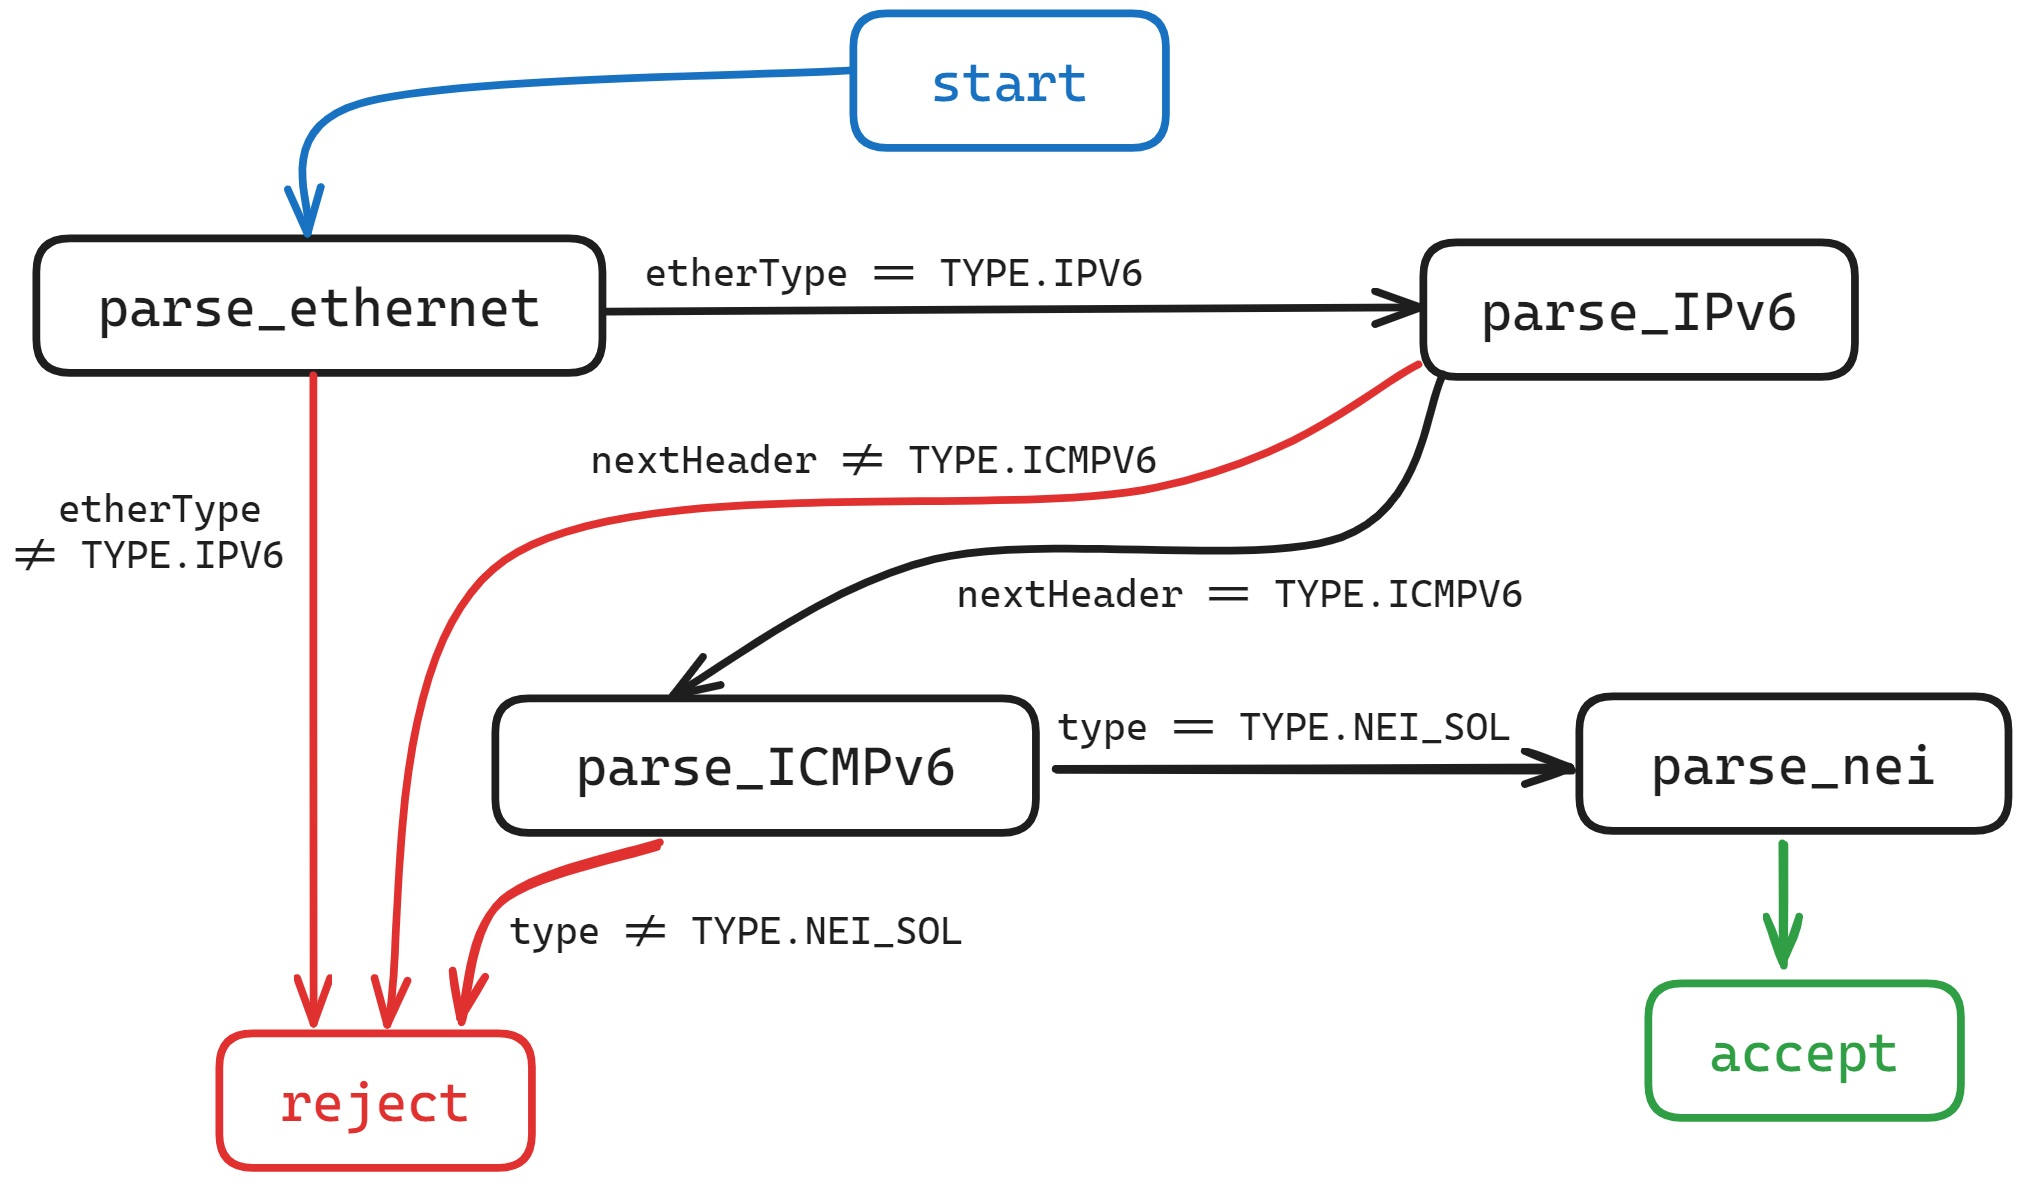
\includegraphics[width=0.60\textwidth]{figures/implementation/ndp_parser.jpg}
     \caption{NDP parser state machine diagram.}
     \label{fig:impl-ndpparser}
\end{figure}

\textbf{Checksum Verification} ~ The ICMPv6 checksum is calculated and verified.

\textbf{Ingress Processing} ~ The router only generates a response if the Hop Limit has not expired, the packet is of type NS, and there is a hit for the target address in the Neighbour Responder table. The control flow for ingress processing is illustrated in \cref{fig:impl-ndpapply}. The NA action constructs an NA packet that contains the link-layer address of the NS's target IPv6 address. The ICMPv6 Type field and the packet flags are updated, the destination addresses set to the original source addresses, and the source addresses set to the router’s respective subnet address. 

\begin{figure}[htbp]
  \centering
    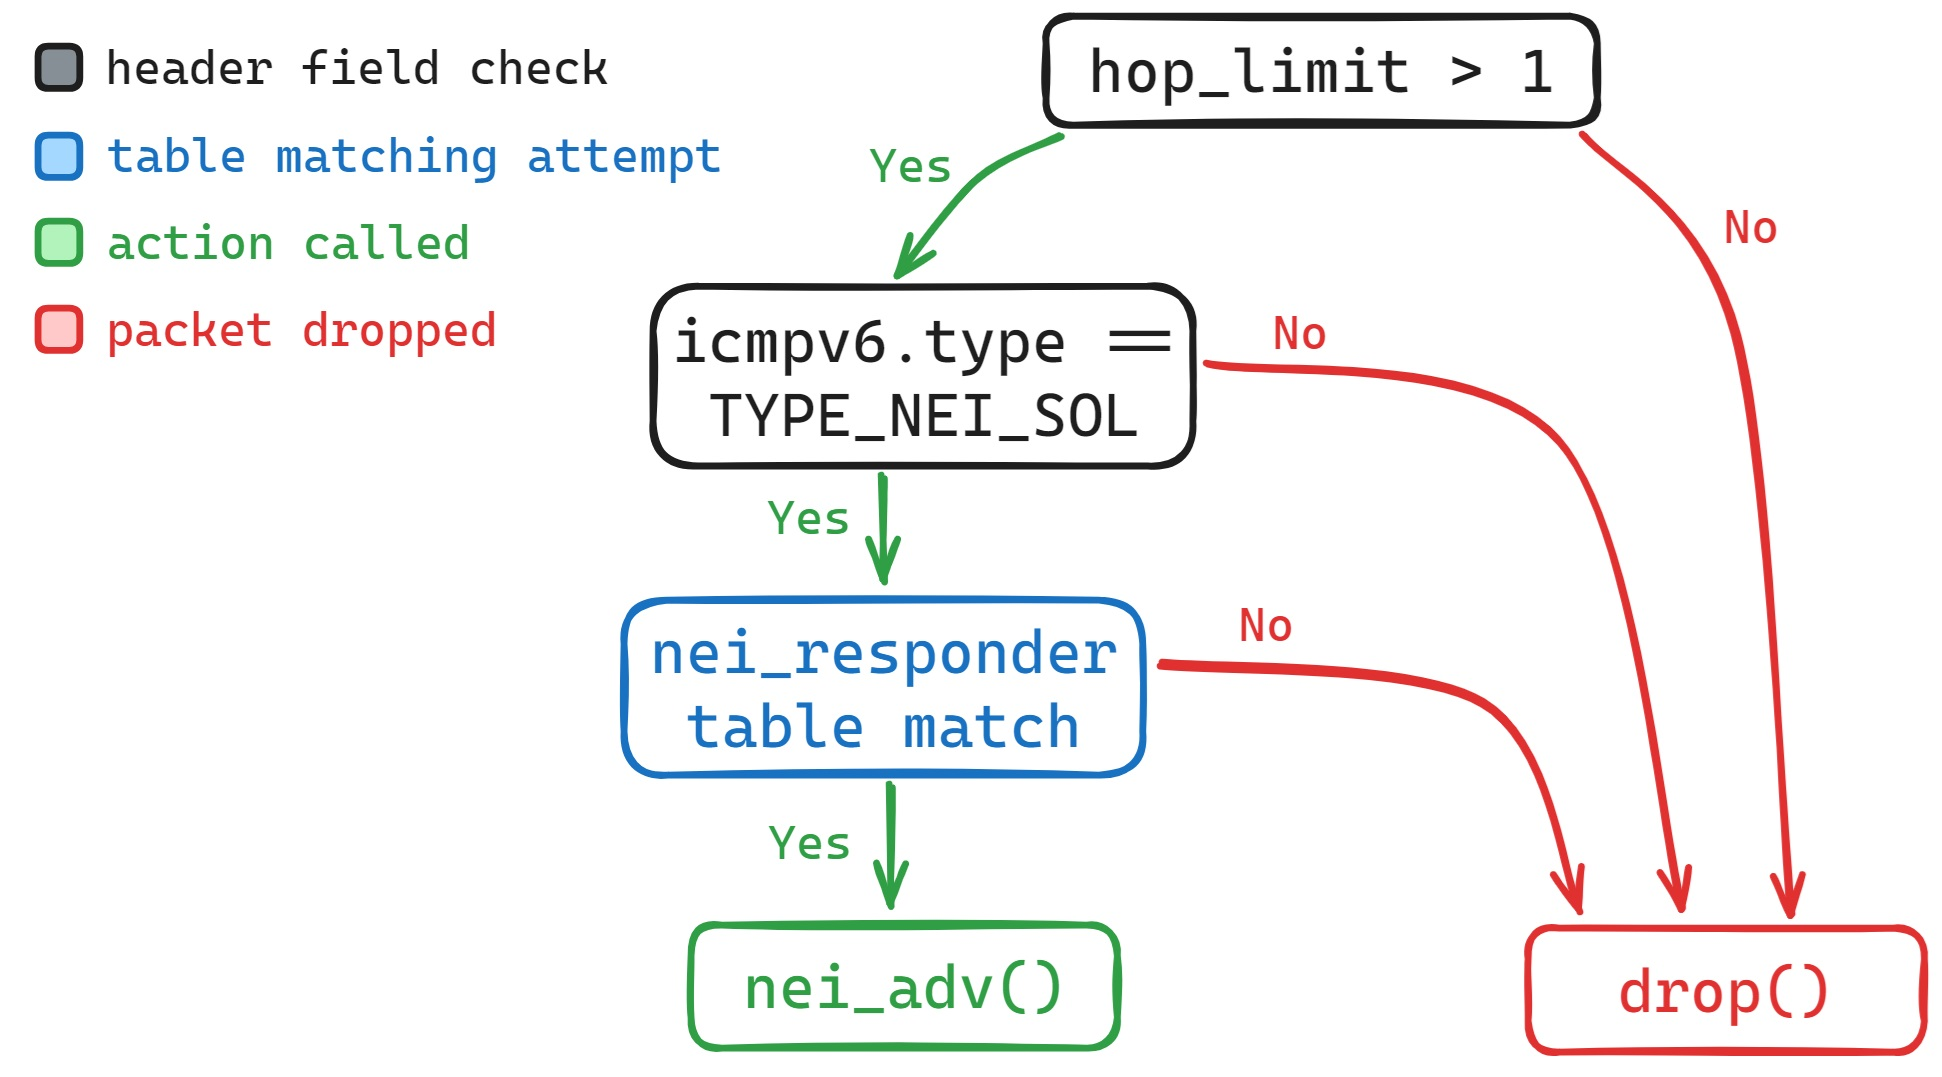
\includegraphics[width=0.65\textwidth]{figures/implementation/ndp_apply.jpg}
     \caption{NDP control flow represented as a simplified decision tree.}
     \label{fig:impl-ndpapply}
\end{figure}

\textbf{Checksum Calculation} ~ The ICMPv6 checksum is calculated and the field updated. 

\textbf{Deparser} ~ The deparser prepends all updated headers and sends the packet to the specified subnet egress port.

This program supports NDP NS and NA functionalities and provides a framework for the implementation to be extended to include other NDP messages. A host sends an NS to the router and receives an NA containing the next-hop MAC address for the target IPv6 address. Hosts can successfully populate their neighbour entry tables through NDP rather than needing manual configuration. This concludes my second project extension.



\section{IPv6 Router}
\label{sec:3.7}

To implement a fully functioning IPv6 router prototype, I combined the functionalities from the three aforementioned sections into one program. My router parses IPv6 packets, checks and updates the Hop Limit, identifies the outbound interface, and forwards the IPv6 packet. Additionally, it responds to Echo Requests and Neighbour Solicitations, and generates Time Exceeded and Destination Unreachable errors, as appropriate.

\subsection{IPv6 Router Design}
\label{sec:3.7.1}

This program supports every functionality outlined in the previous three sections. The code for \texttt{router6.p4} is built by combining the \texttt{ipv6.p4}, \texttt{icmpv6.p4}, and \texttt{ndp.p4} programs. For more detailed information on how to run this experiment, consult Appendix F.

\subsection{IPv6 Router Program}
\label{sec:3.7.2}

The data plane behaviour of the router is defined by the P4 file \texttt{router6.p4}.

\textbf{Header Definitions} ~ All headers defined in \cref{sec:3.4}, \cref{sec:3.5}, and \cref{sec:3.6} are included. A header union is defined to combine the Echo and the Nei headers, as they are both encapsulated within the ICMPv6 payload.

\textbf{Parser} ~ This program's parser merges the respective parsers of the individual functionalities. All intermediate states have been added and additional branches defined when multiple transitions are possible. As before, any packet that is not of type IPv6 gets rejected. Every ICMPv6 packet gets accepted and, if it is identified as an Echo Request or an NS packet, the additional headers also get parsed, as shown in \cref{fig:impl-router6parser}.

\begin{figure}[htbp]
  \centering
    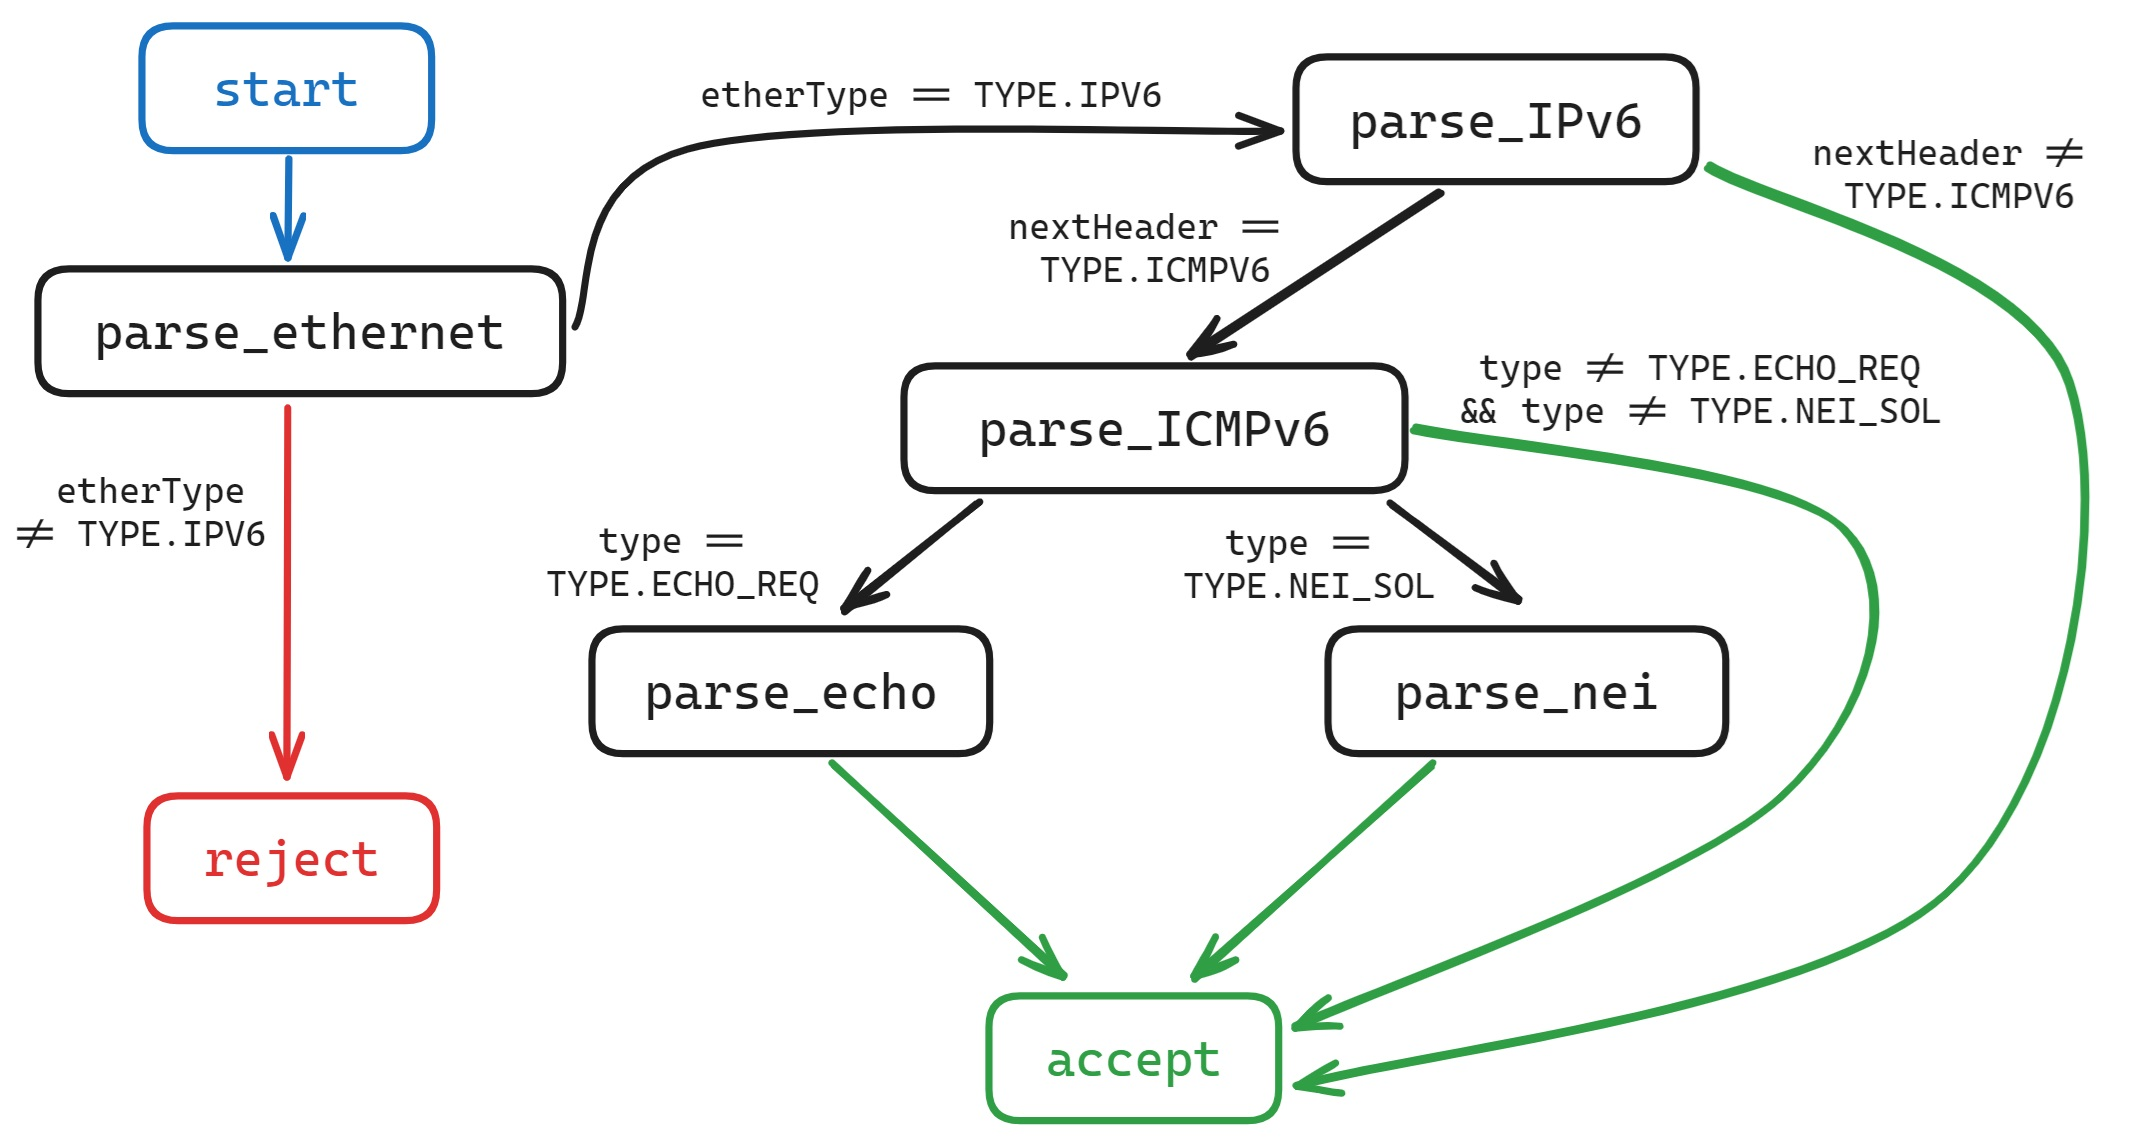
\includegraphics[width=0.85\textwidth]{figures/implementation/router6_parser.jpg}
     \caption{IPv6 router parser state machine diagram.}
     \label{fig:impl-router6parser}
\end{figure}

\textbf{Checksum Verification} ~ Depending on the packet type and destination, the ICMPv6 Checksum field may be verified. IPv6 packets that are only forwarded by the router do not have their payloads inspected. Echo Request packets directed towards the router or NS packets (regardless of their destination address, usually a node multicast address) have their checksums verified.

\textbf{Ingress processing} ~ The application block integrates the three separate control flows. First and foremost, if the Hop Limit is less than or equal to one, the Time Exceeded action is triggered. Otherwise, the program checks whether the packet is an Echo Request or an NS. If it is, the target address gets matched in the corresponding table and, in case of a match, the respective action is called. If it is an Echo Request packet whose destination address is not the router, the router checks for a match in the forwarding table. If it is an NS packet without a match in the Neighbour Responder table, it is dropped.

The router will attempt to forward any other IPv6 packet based on its destination address by performing a longest prefix match on the packet's destination address. If a match is found, the forwarding action is called, and the next hop MAC address and egress ports are defined.  If there is no match in the IPv6 forwarding table, a Destination Unreachable error message is generated. \cref{fig:impl-router6apply} illustrates the described control flow. All individual actions in the program are identical to the ones previously described.

\begin{figure}[htbp]
  \centering
    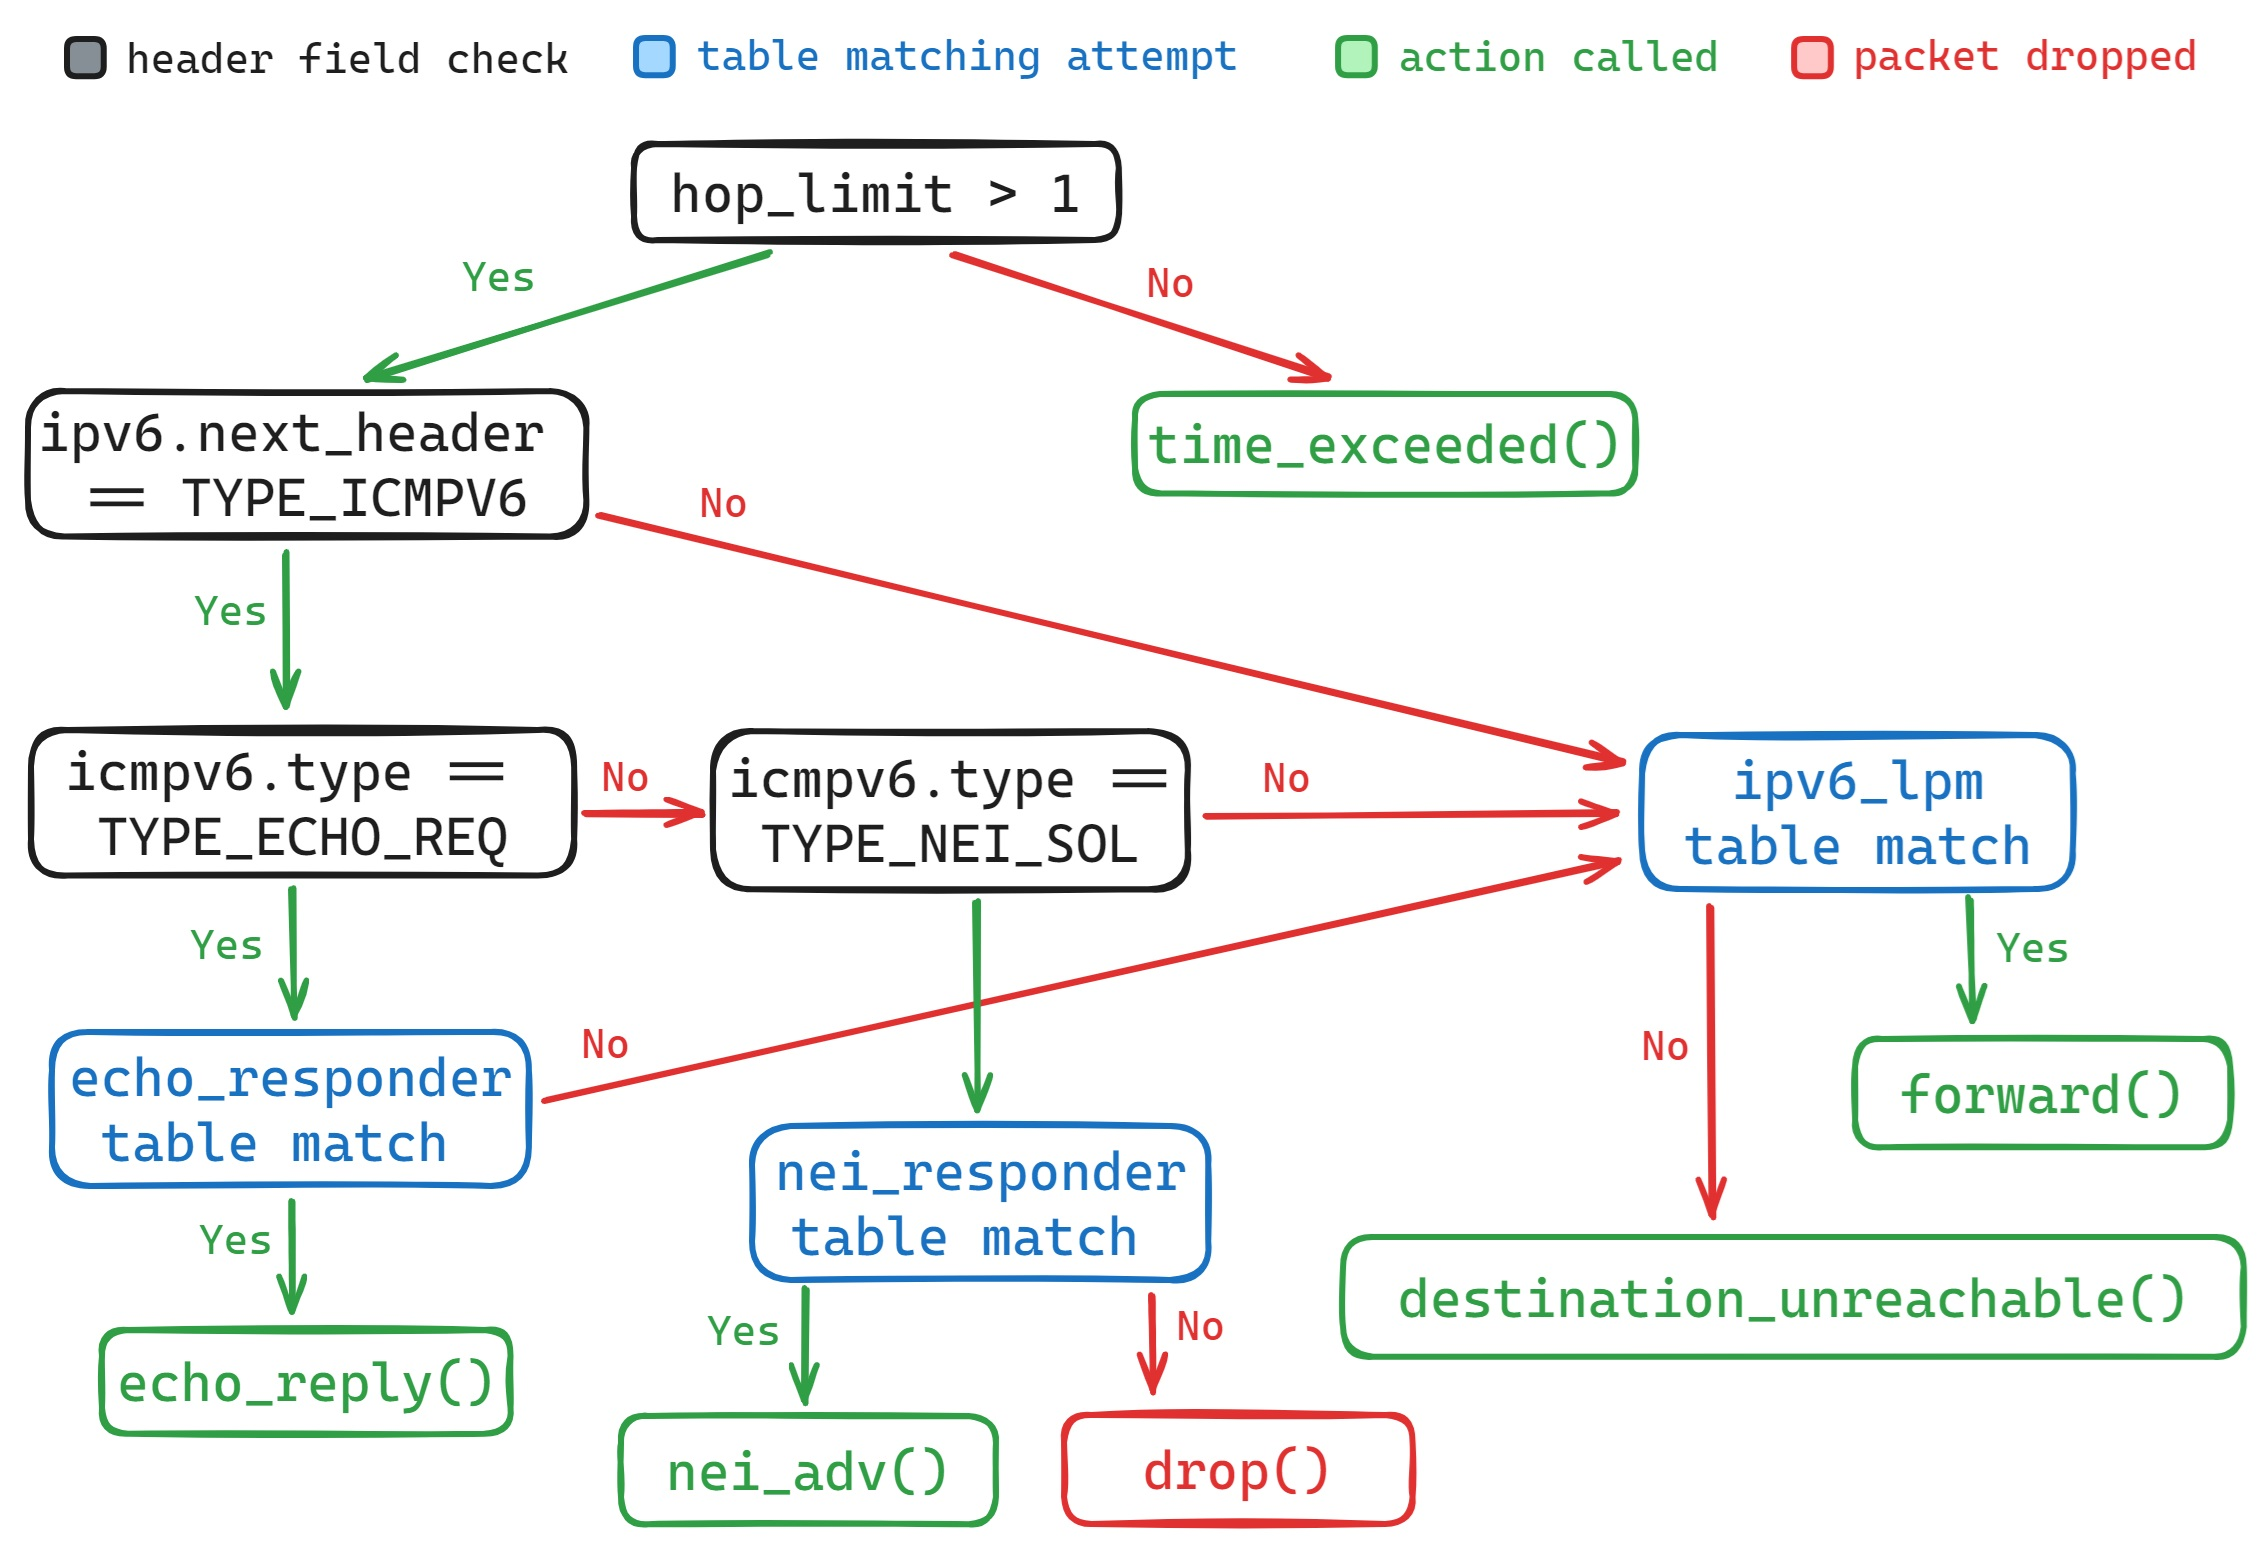
\includegraphics[width=0.9\textwidth]{figures/implementation/router6_apply.jpg}
     \caption{IPv6 router control flow represented as a simplified decision tree.}
     \label{fig:impl-router6apply}
\end{figure}

\textbf{Checksum Calculation} ~ If a response packet is generated (Echo Reply, NA, or an ICMPv6 error message), then an ICMPv6 checksum is calculated and the field updated. Otherwise, no checksum calculation is performed.

\textbf{Deparser} ~ The deparser prepends any relevant headers based on the action that has been triggered and sends the packet through the specified egress port.

This program implements IPv6 packet parsing and forwarding with the use of a longest prefix destination address matching. The router responds to Echo Requests with Echo Replies and to NSs with NAs. It also generates Time Exceeded and Destination Unreachable error messages, when appropriate. The hosts in the network can establish a connection through the router and begin to exchange packets. They can also check router availability and are made aware if a packet's Hop Limit has expired or if the router cannot find a path to the IPv6 address they are trying to reach. The program has been written such that it can easily be extended to support other ICMPv6 and NDP functionalities.


\section{Support for Both IPv4 and IPv6}
\label{sec:3.8}

As the Internet continues to grow, the adoption of IPv6 becomes more unavoidable. Currently, there exist nodes on the network which support only IPv4 or only IPv6. These nodes might still want to communicate with each other, or might need to route packets through each other to reach other nodes, and the network must be able to support these interactions. To aid in the transition from IPv4 to IPv6, mechanisms for a network to support both IPv4 and IPv6 nodes have been introduced, most notably translation, tunneling, and dual IP layering. In this section I describe all three mechanisms and explain why I chose dual IP layering for the final stage of my project.

\subsection{Translation}
\label{sec:3.8.1}

Translation of IP addresses was invented to allow hosts using the two different IPs to communicate. This mechanism depends on the existence of Address Family Border Routers (AFBRs) in the network, whose job is to translate addresses from one protocol to the other. Hosts that want to communicate with each other need to first acquire each other's aliased addresses \cite{TransitionsPaper}. For example, \cref{fig:impl-translation} depicts Host 1, using IPvX, who directs a packet towards an alias `IPvX address'. Upon reaching the AFBR, this packet gets transformed into an IPvY packet and both addresses get updated. The source address of the IPvX host is updated to its alias `IPvY address' and the destination address to its real IPvY address.

\begin{figure}[htbp]
  \centering
    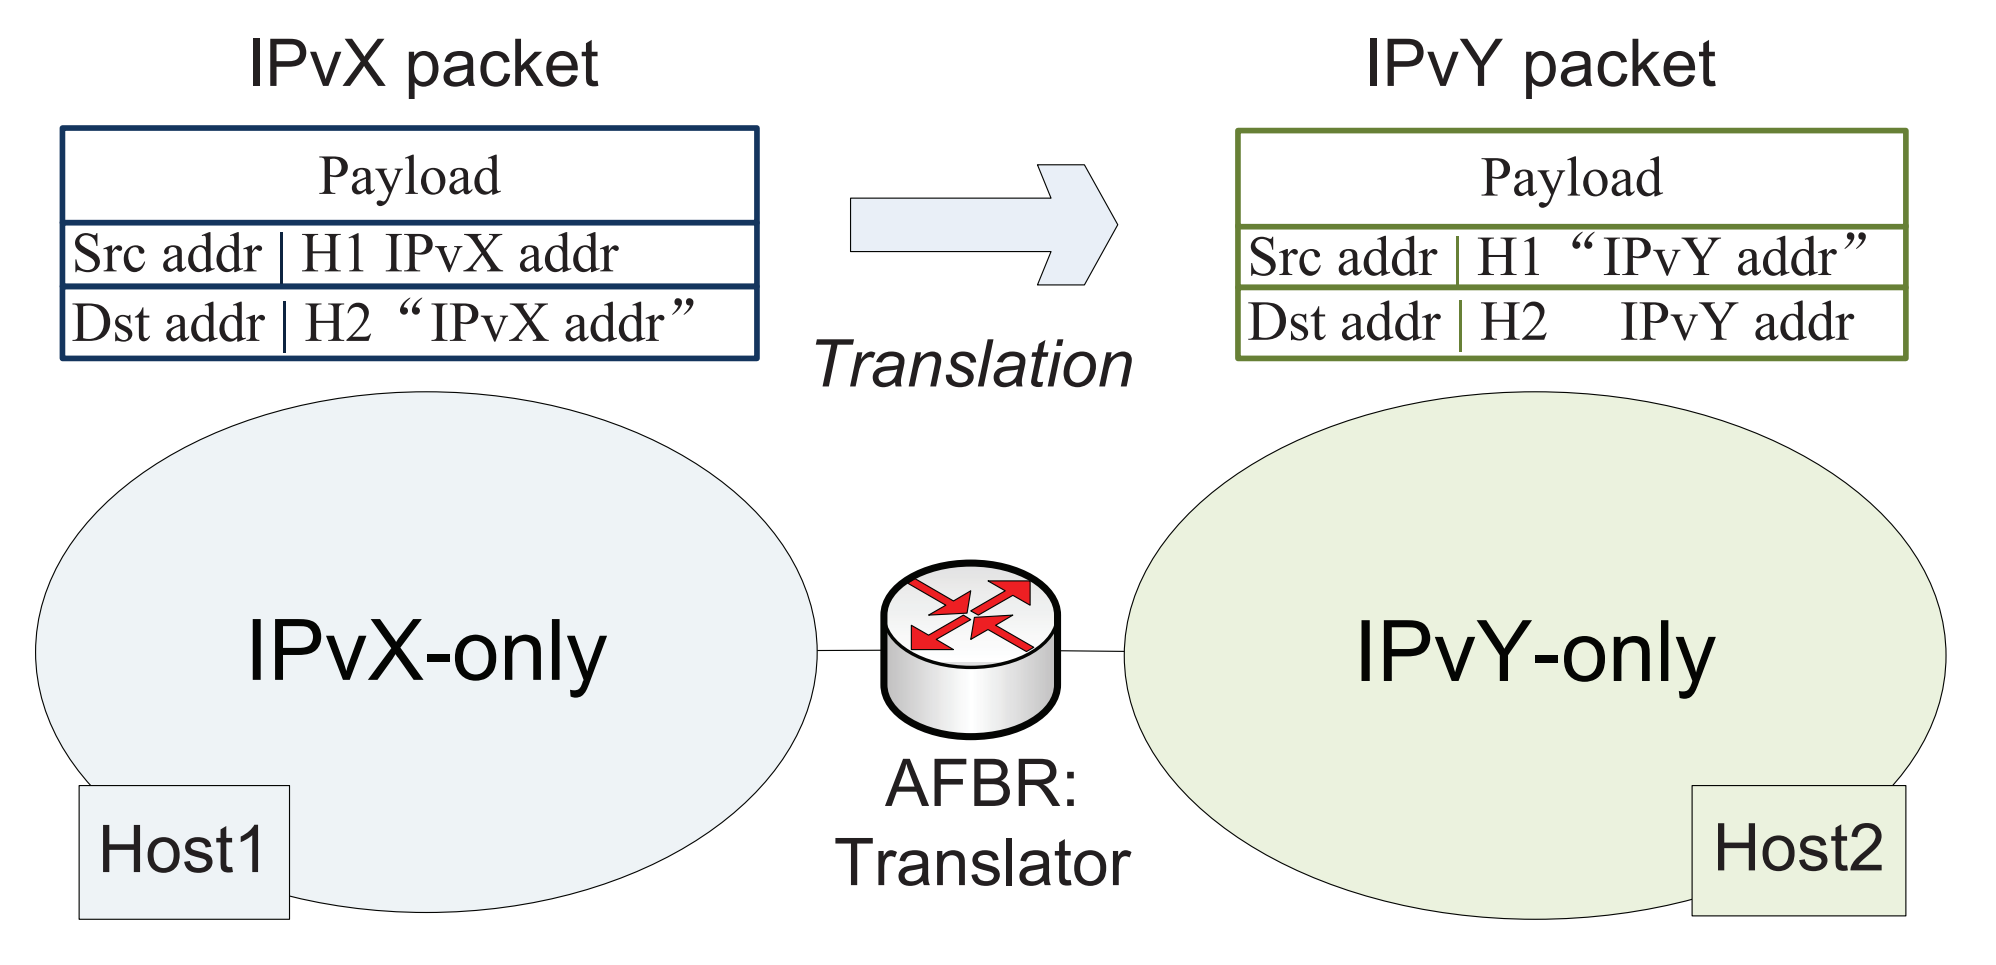
\includegraphics[width=0.5\textwidth]{figures/implementation/translation.png}
     \caption{IP translation. Taken from \cite{TransitionsPaper}.}
     \label{fig:impl-translation}
\end{figure}

The translation mechanism faces many challenges, such as guaranteeing the packet passes through an AFBR along its route; how AFBR mapping assignments are assigned; conversion of upper layer header fields (such as ICMP/TCP/UDP fields), essentially violating the end-to-end network principle; fragmentation and reassembly; and many others \cite{TransitionsPaper}. Translation does not scale well and poses many issues for networks that rely on it to support both IPs.



\subsection{Tunneling}
\label{sec:3.8.2}

Tunneling of IP packets is a mechanism used when a packet whose two end hosts use the same IP needs to pass through a portion of the network that uses a different IP \cite{Tunneling}. At the transition point between the two IP networks, an entry node encapsulates the packet by prepending a temporary IP header and leaving the original packet as a payload. The exit node removes this temporary header and forwards the packet onwards, as shown in \cref{fig:impl-tunneling} \cite{Tunneling}.

\begin{figure}[htbp]
  \centering
    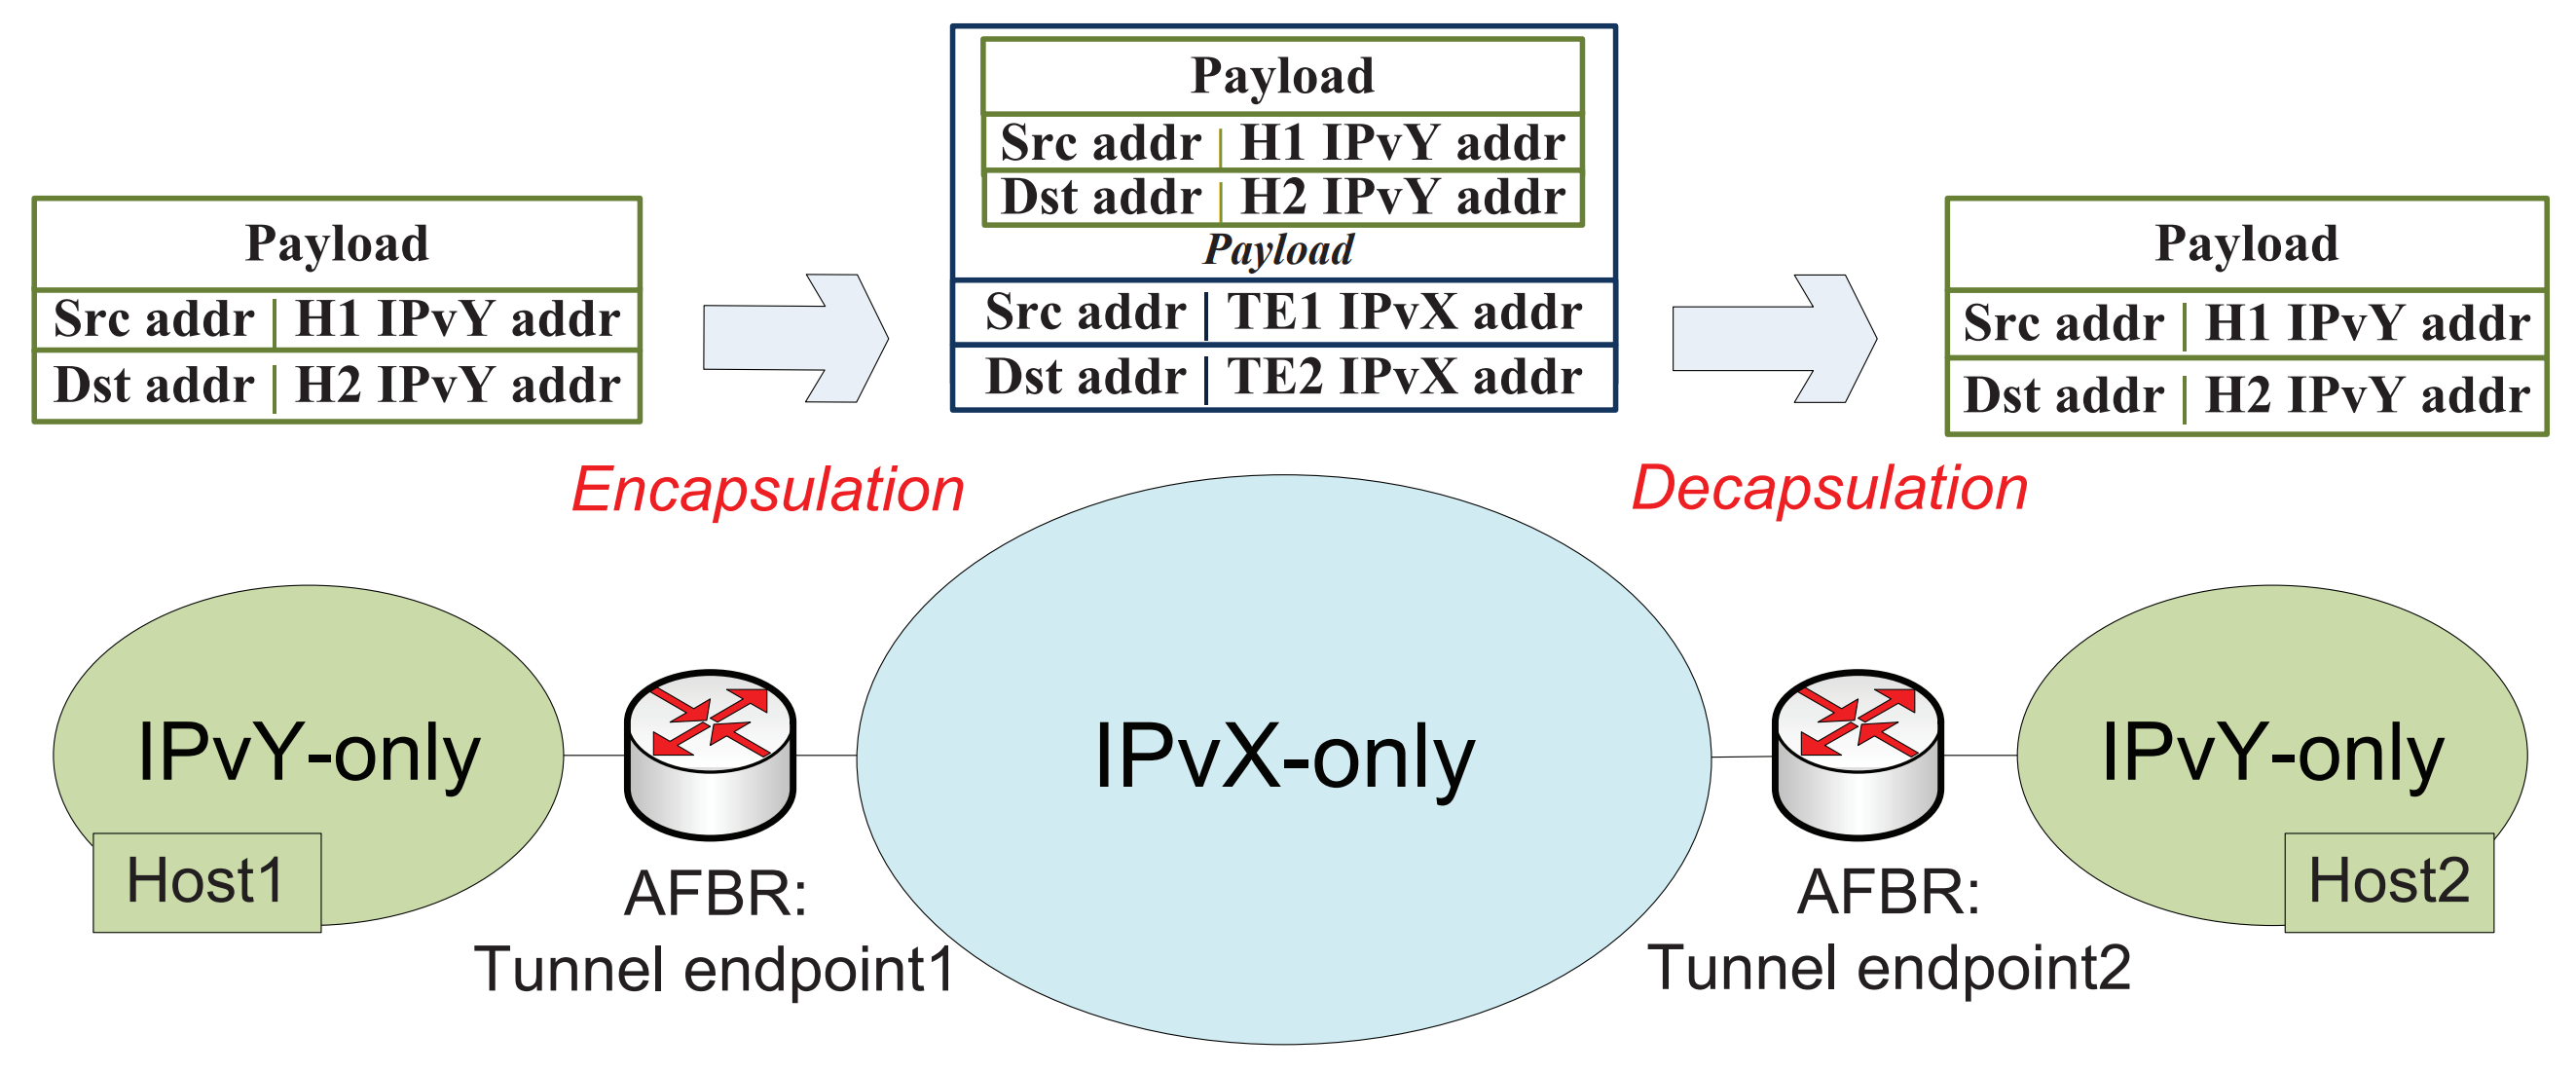
\includegraphics[width=0.6\textwidth]{figures/implementation/tunneling.png}
     \caption{IP tunneling. Taken from \cite{TransitionsPaper}.}
     \label{fig:impl-tunneling}
\end{figure}

Although tunneling is a simpler mechanism, it still faces challenges. Different types of encapsulation are required depending on the taken route, packets may need to be fragmented if they exceed the maximum size of the tunneling network, and NATs and firewalls encountered along the way may not be configured to handle encapsulated packets \cite{TransitionsPaper}.



\subsection{Dual IP Layering}
\label{sec:3.8.3}

The dual IP approach to network nodes implements two fully independent stacks, one for each IP, side-by-side. It supports separate network interfaces such that the node can identify and process both IPv4 and IPv6 \cite{DualStack}. A dual-stacked node can communicate with both IPv4 nodes and IPv6 nodes. Either stack can continue functioning even if the other is disabled \cite{DualStackSpecs}.

The dual IP approach does little to solve the IPv4 address exhaustion problem, as it still requires that a node has an IPv4 address. It does, however, ease the transition from IPv4 to IPv6 by providing separate implementations for both protocols and supporting communication with both types of nodes, and is becoming more and more widespread as IPv6 adoption is increasing \cite{DualStack}. 

For this project, I decided to provide support for both IPs by extending my IPv6 router to incorporate an IPv4 router implementation. This approach enables maximum flexibility of the node, whilst also allowing me to evaluate the functional correctness of individual IP implementations.



\section{Dual-Stack Router}
\label{sec:3.9}

My third extension is to implement support for both IPv4 and IPv6 packets. I do this by building a dual-stack router prototype. I use the IPv6 router I already built, as defined in \cref{sec:3.7}. In \cref{sec:3.9.1} I describe building a simple IPv4 router. In the remainder of this section, I explain the process of merging the two prototypes to bring to fruition a router that supports both IPv4 and IPv6.



\subsection{IPv4 Router}
\label{sec:3.9.1}

In order to obtain an IPv4 router prototype, I combine the functionalities available in the P4Pi repository into a single program, \texttt{router.p4}. There were separate P4 programs that implemented IPv4 forwarding, ARP neighbour discovery, and ICMPv4 Echo Request/Reply. Similarly to how I implemented the IPv6 router, I build a program that defines all necessary header types, combines the parser state machines and merges the ingress processing control flows. The Destination Unreachable and Time Exceeded functionalities are additional features that my IPv6 router prototype supports, but that were not included in the original IPv4 functionalities.



\subsection{Dual-Stack Router Design}
\label{sec:3.9.2}

Each host now has two IP addresses (an IPv4 and an IPv6 address) and two MAC address tables (one for ARP and one for NDP). Correspondingly, the router now has four statically defined addresses: two for each subnet. All tables in the P4 program are populated dynamically using the CLI. For more information on how to run this experiment, consult Appendix G. The program can parse and forward both IPv4 and IPv6 packets, respond to Echo Requests in both IPs, and match IP addresses to next-hop MAC addresses using ARP or NDP. On the IPv6 stack, ICMPv6 also supports two error messages.



\subsection{Dual-Stack Router Program}
\label{sec:3.9.3}

The data plane behaviour of the router is defined by the P4 file \texttt{dualstack.p4}.

\textbf{Header Definitions} ~ The \texttt{dualstack.p4} program defines a total of seven headers: Ethernet, ARP, IPv4, IPv6, ICMP, Echo, and Nei. 

\textbf{Parser} ~ The parser state machine only accepts packets that start with an Ethernet frame. It then checks the next header. ARP packets are accepted if they are an ARP Request. IPv4 and IPv6 packets are accepted regardless of what they contain, but checks are still performed in case they are ICMP packets to make sure all relevant headers are extracted. The parser’s state machine can be seen in \cref{fig:impl-dualparser}.

\begin{figure}[htbp]
  \centering
    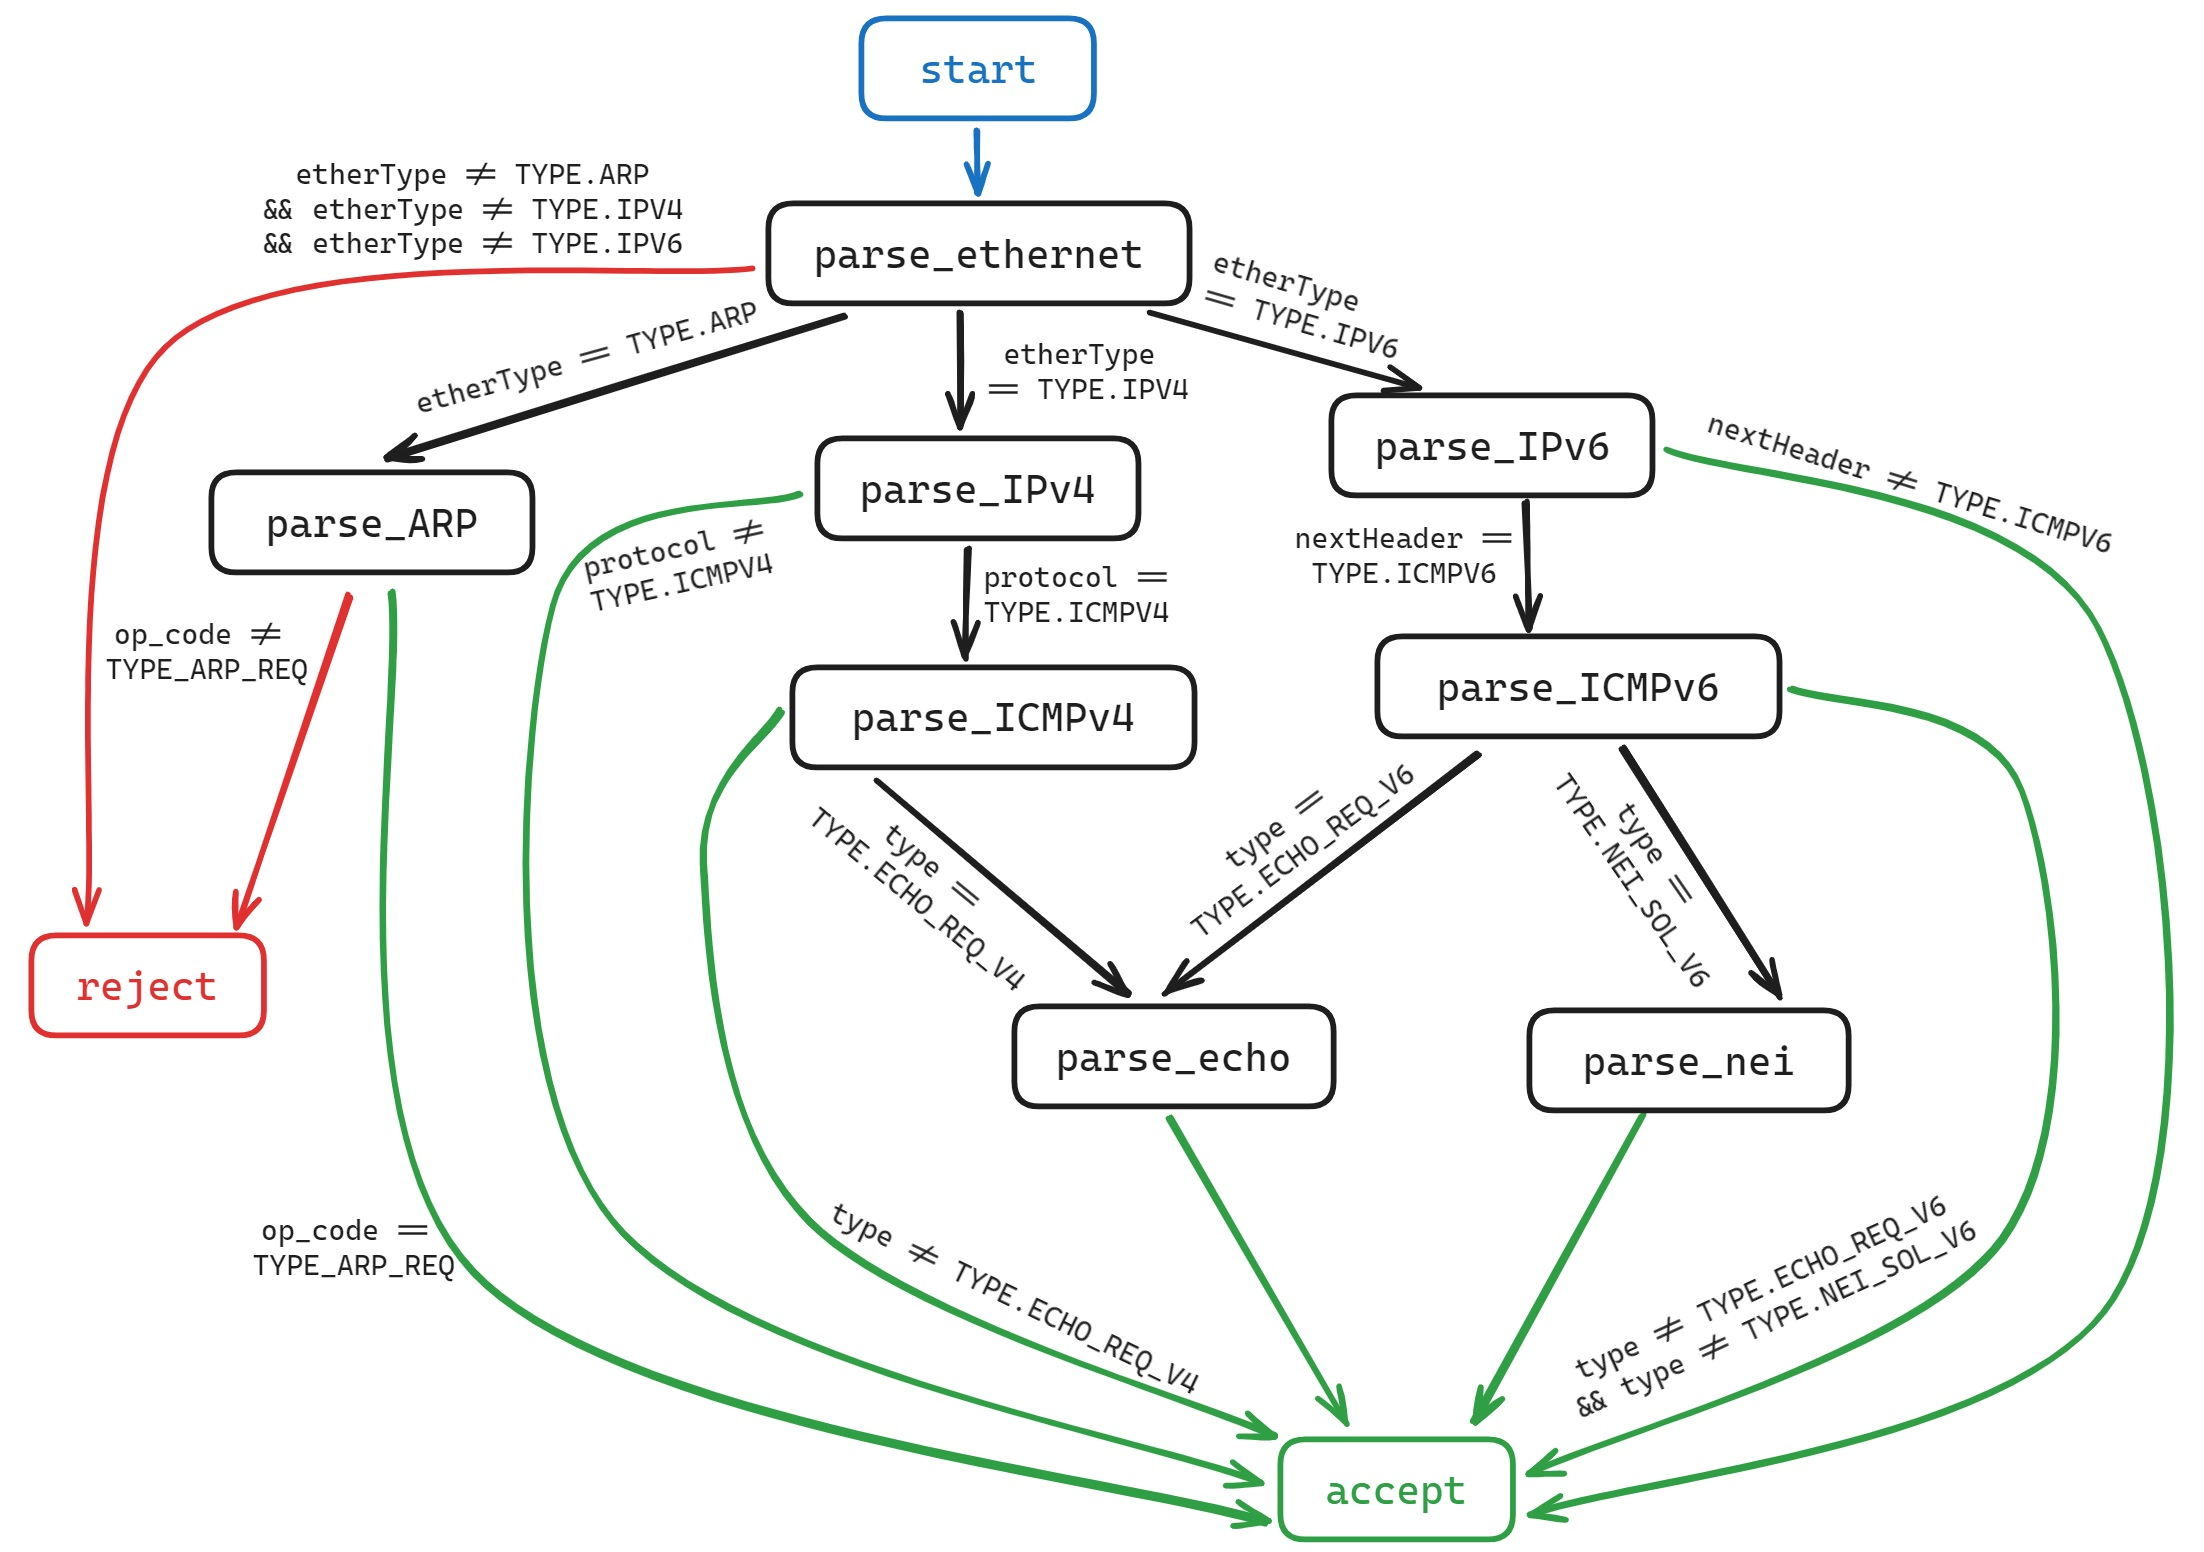
\includegraphics[width=1\textwidth]{figures/implementation/dualstack_parser.jpg}
     \caption{Dual-stack router parser state machine diagram. A packet is accepted \\ if it is of type IPv4, IPv6, or an ARP Request.}
     \label{fig:impl-dualparser}
\end{figure}

\textbf{Checksum Verification} ~ IPv4, ICMPv4 and ICMPv6 checksums are calculated and verified. Packets that are of type IPv6 and only get forwarded to their next-hop destination do not have any checksums verified.

\textbf{Ingress Processing} ~ The ingress processing of the dual-stack router represents the merging of the two control flows of the IPv4 router and the IPv6 router. If it is an ARP Request, the program looks for a match in the ARP table. If there is a hit, an ARP Reply packet is generated, containing the MAC address of the requested IPv4 address. If there is no match in the table, the packet gets dropped. If the packet has an IPv4 header, its Time To Live field gets checked first: if it is zero or one, the packet gets dropped because the IPv4 router does not have Time Exceeded error message functionality; if it is larger than one, the router checks whether the packet is an Echo Request directed towards the router. If it is, an Echo Reply is generated. Otherwise, the packet gets forwarded using an IPv4 longest prefix match table. If the packet is of type IPv6, it enters the control flow that was described in the \cref{sec:3.7}. In the end, every packet is either forwarded, dropped, an informational response is generated, or an error message is triggered. 

\begin{figure}[htbp]
  \centering
    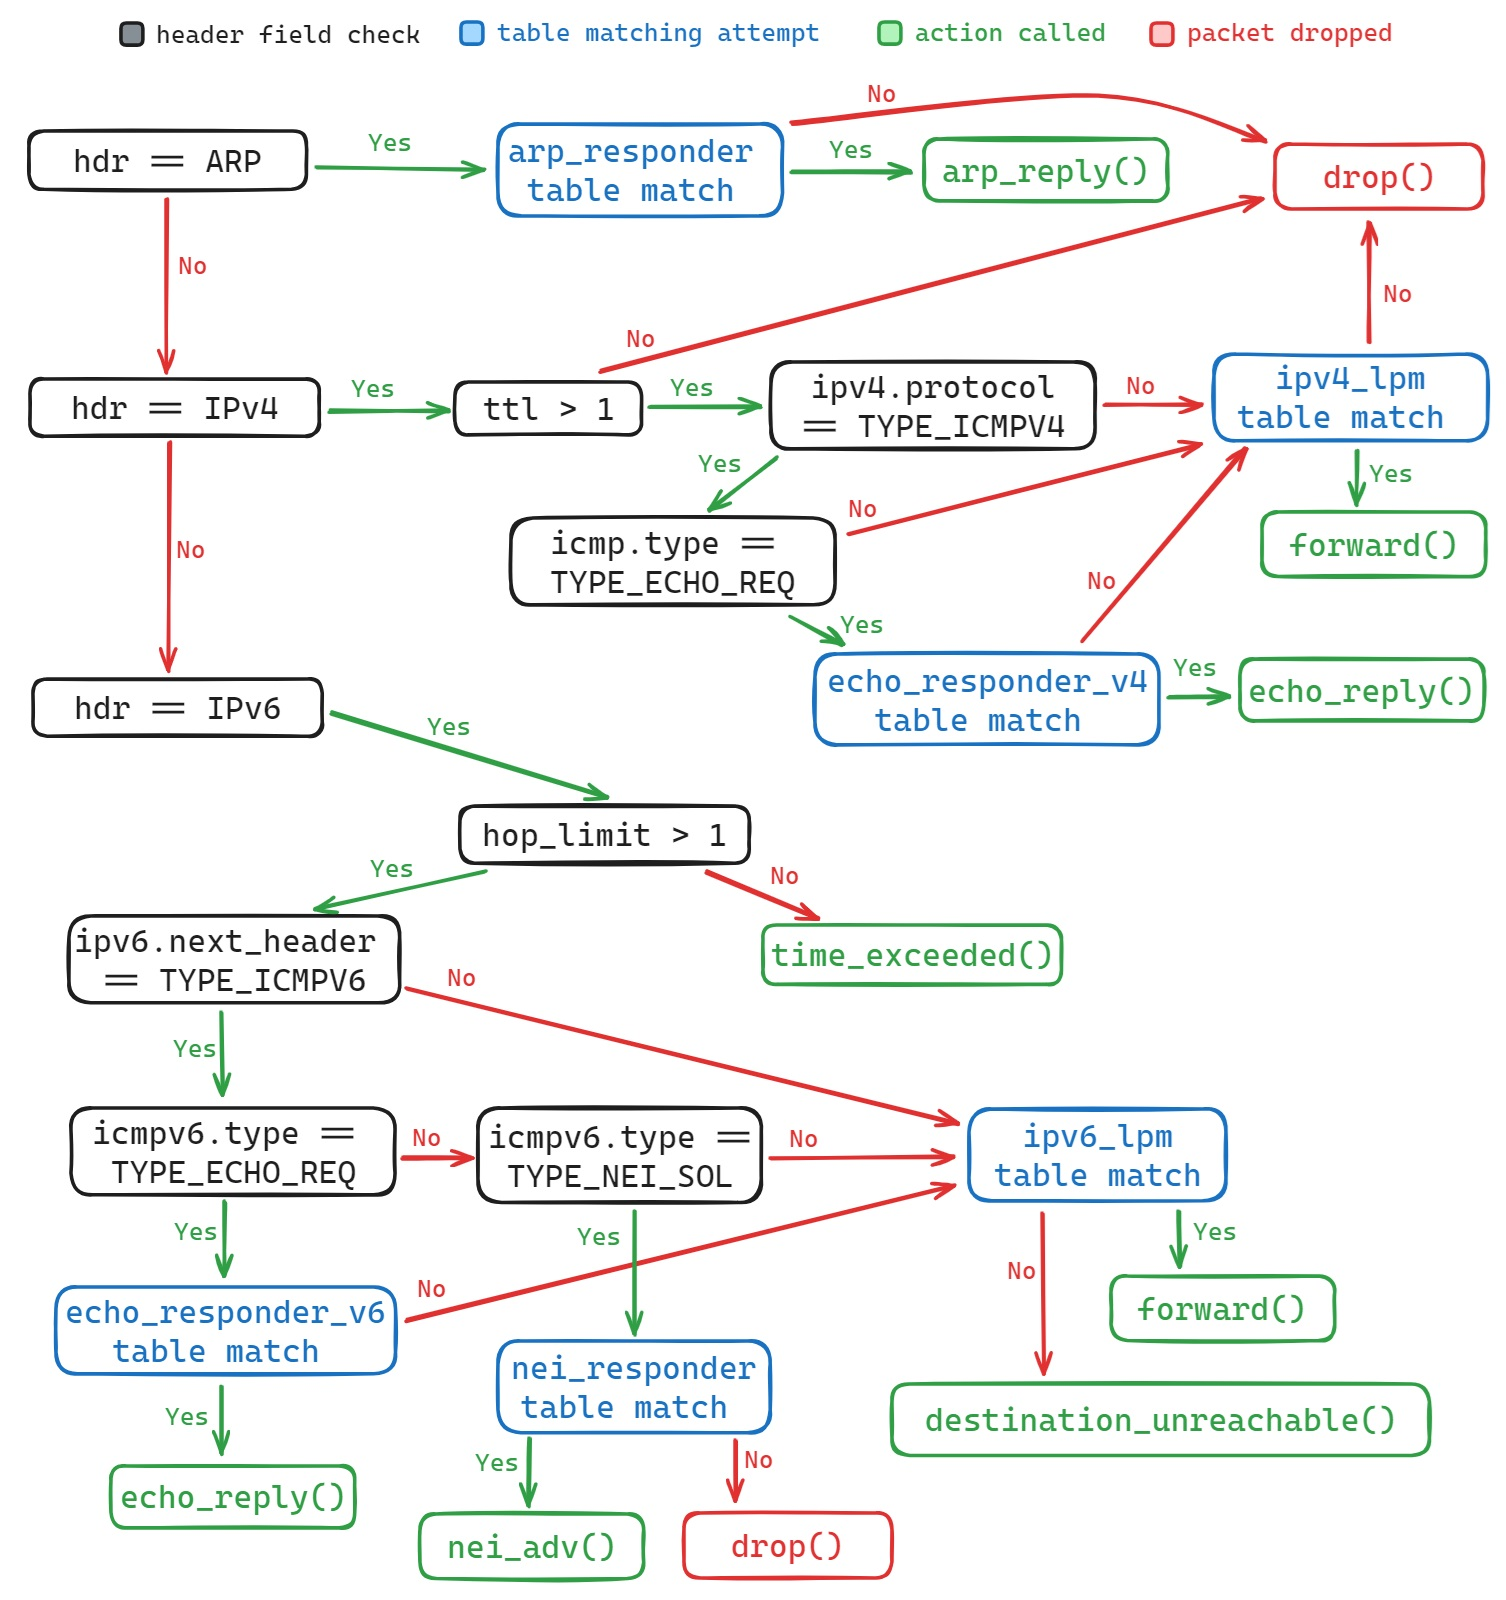
\includegraphics[width=1\textwidth]{figures/implementation/dualstack_apply.jpg}
     \caption{Dual-stack router control flow represented as a simplified decision tree.}
     \label{fig:impl-dualapply}
\end{figure}

\cref{fig:impl-dualapply} illustrates the dual-stack router's more complex control flow. Some of the action blocks have been duplicated to avoid overcomplicating the diagram. Any two blocks that share the same name refer to the same functionality. Notice the lack of a red arrow leaving the `\texttt{hdr == IPv6}' block. This is because if the packet does not match either an ARP, an IPv4 or an IPv6 header, it never would have passed the parser stage, so it must follow the green arrow out of that block.

\textbf{Checksum Calculation} ~ Any necessary IPv4, ICMPv4 or ICMPv6 checksums are recalculated and their corresponding field is updated.

\textbf{Deparser} ~ Depending on the action that was selected, the relevant headers are prepended, and the reconstructed packet is sent out the specified egress port.

This program implements both IPv4 and IPv6 forwarding, along with both ICMPv4 and ICMPv6 Echo Request/Reply. It also supports IPv4 ARP and ICMPv6 NDP. Two additional error messages are supported by ICMPv6. Hosts in the network can discover next-hop MAC addresses and exchange packets in both IPs.


\section{Implementation Summary}
\label{sec:3.10}

In this chapter I described the implementation process of building individual IPv6 router functionalities and integrating them into a fully-functional IPv6 router prototype. Every program abides by the \textit{V1Model} architecture model and defines distinct code blocks that correspond to the architecture pipeline stages. All configurations run on the \textit{simple switch} target and use the \textit{simple switch CLI} to populate the data plane tables. The functionalities were designed to mimic the packets exchanged with a working home router. As my final extension, I add an IPv4 stack in order to create a dual-stack router prototype that supports packets in both IPs. By completing these tasks, I have achieved all of my project's core objectives, along with three of the proposed extensions.